\documentclass{sfuthesis}

\title{Bilingual Language Models using Word Embeddings for Machine Translation}
\thesistype{Thesis}
\author{Jasneet Singh Sabharwal}
\previousdegrees{%
	B.Tech., Guru Gobind Singh Indraprastha University, 2010}
\degree{Master of Science}
\discipline{Computing Science}
\department{School of Computing Science}
\faculty{Faculty of Applied Sciences}
\copyrightyear{2016}
\semester{Summer 2016}
\date{19 May 2016}

\keywords{Bilingual Language Models; Bilingual Word Embeddings; Machine Translation}

\committee{%
	\chair{Ryan Shea}{University Research Associate - Big Data Systems\\Simon Fraser University}
	\member{Anoop Sarkar}{Co-Senior Supervisor\\Professor, School of Computing Science\\Simon Fraser University}
	\member{Fred Popowich}{Co-Senior Supervisor\\Professor, School of Computing Science\\Simon Fraser University}
	\member{Jiannan Wang}{Internal Examiner\\Assistant Professor, School of Computing Science\\Simon Fraser University}
}

%   PACKAGES AND CUSTOMIZATIONS  %%%%%%%%%%%%%%%%%%%%%%%%%%%%%%%%%%%%%%%%%%%%%%
%
%   Add any packages or custom commands you need for your thesis here.
%   You don't need to call the following packages, which are already called in
%   the sfuthesis class file:
%
%   - appendix
%   - etoolbox
%   - fontenc
%   - geometry
%   - lmodern
%   - nowidow
%   - setspace
%   - tocloft
%
%   If you call one of the above packages (or one of their dependencies) with
%   options, you may get a "Option clash" LaTeX error. If you get this error,
%   you can fix it by removing your copy of \usepackage and passing the options
%   you need by adding
%
%       \PassOptionsToPackage{<options>}{<package>}
%
%   before \documentclass{sfuthesis}.
%

\usepackage{amsmath,amssymb,amsthm}
\usepackage[pdfborder={0 0 0}]{hyperref}
\usepackage{graphicx}
\usepackage{caption}
\usepackage{boxedminipage}
\usepackage{breakcites}
\usepackage{multirow}
\usepackage{xeCJK}
\NewDocumentCommand{\textzh}{m}{%
	\begingroup\makexeCJKactive#1\endgroup
}



%   FRONTMATTER  %%%%%%%%%%%%%%%%%%%%%%%%%%%%%%%%%%%%%%%%%%%%%%%%%%%%%%%%%%%%%%
%
%   Title page, committee page, copyright declaration, abstract,
%   dedication, acknowledgements, table of contents, etc.
%

\begin{document}

\frontmatter
\maketitle{}
\makecommittee{}


%% Copyright 1998 Pepe Kubon
%%
%% `abstract.tex' --- abstract for thes-full.tex, thes-short-tex from
%%                    the `csthesis' bundle
%%
%% You are allowed to distribute this file together with all files
%% mentioned in READ.ME.
%%
%% You are not allowed to modify its contents.
%%

%%%%%%%%%%%%%%%%%%%%%%%%%%%%%%%%%%%%%%%%%%%%%%%%%
%
%       Abstract 
%
%%%%%%%%%%%%%%%%%%%%%%%%%%%%%%%%%%%%%%%%%%%%%%%%

\begin{abstract}
Bilingual language models(Bi-LMs) refers to language models that are modeled using both source and target words in a parallel corpus. While translating a source sentence to a target language, the decoder in phrase-based machine translation system breaks down the source sentence into phrases. It then translates each phrase into the target language. While decoding each phrase, the decoder has very little information about source words that are outside the current phrase in consideration. Bi-LMs have been used to provide more information about source words outside the current phrase. Bi-LMs are estimated by first creating bitoken sequences using a parallel corpus and the word alignments between the source and target words in that corpus. When creating the bitoken sequences, the vocabulary expands considerably and Bi-LMs suffer due to this huge vocabulary which in turn increases the sparsity of the language models. In previous work, bitokens were created by first replacing each word in the parallel corpus either by their part-of-speech tags or word classes after clustering using Brown clustering algorithm. Both of these approaches only take into account words that are direct translations of each other as they only depend on word alignments between the source word and target word in the bitokens. We propose to use bilingual word embeddings to reduce the vocabulary of the bitokens. Bilingual word embeddings are a low dimensional representation of words in two languages such that words in either language that are similarly distributed are placed nearby in an abstract vector space. Our approach outperforms previous work using Bi-LMs with an increase of 1.4 BLEU points in our experiments.
\end{abstract}
%%% Copyright 1998 Pepe Kubon
%%
%% `dedquot.tex' --- dedication and quotation for thes-full.tex from
%%                   the `csthesis' bundle
%%
%% You are allowed to distribute this file together with all files
%% mentioned in READ.ME.
%%
%% You are not allowed to modify its contents.
%%

%%%%%%%%%%%%%%%%%%%%%%%%%%%%%%%%%%%%%%%%%%%%%
%
%   Dedication/Quotation pages
%
%%%%%%%%%%%%%%%%%%%%%%%%%%%%%%%%%%%%%%%%%%%%%

\begin{dedication} % optional
	To Mom and Dad!
\end{dedication}
%%% Copyright 1998 Pepe Kubon
%%
%% `ack.tex' --- Acknowledgements for thes-full.tex, thes-short-tex from
%%               the `csthesis' bundle
%%
%% You are allowed to distribute this file together with all files
%% mentioned in READ.ME.
%%
%% You are not allowed to modify its contents.
%%

%%%%%%%%%%%%%%%%%%%%%%%%%%%%%%%%%%%%%%%%%%%
%
%       Acknowledgement
%
%%%%%%%%%%%%%%%%%%%%%%%%%%%%%%%%%%%%%%%%%%

\begin{acknowledgements} % optional
\begin{itemize}
	\item Anoop - for everything, all the help and support that he has provided. This thesis wouldn't be there without him.
	\item Fred - for being supportive in my endeavours.
	\item Hieu Hong and Kenneth Heafield - for helping me out with moses
	\item George Foster, Darlene Stewart, Roland Kuhn and Eric Joanis - for helping me out in setting up the baseline
	\item Karl Moritz Hermann - for helping me out with embeddings
	\item Milica - for being there for me, for all the snores and sleepless nights
	\item Rejaa - aive hee for all the laughs and fun times
	\item Brad, Rohit and Diljot - for being supportive and helping me out in Canada
	\item Anahita - for being cheerful and hopeful
	\item Maryam - for the datasets
	\item Gladys and Carolyn - for immense support and helping me out even before i came to canada
	\item Amir and Jeanette - for all the love and support
	\item Te Bu - for looking at bilingual word embeddings and helping us to get the best parameters.
\end{itemize}
\end{acknowledgements}


\addtoToC{Table of Contents}\tableofcontents\clearpage
\addtoToC{List of Tables}\listoftables\clearpage
\addtoToC{List of Figures}\listoffigures





%   MAIN MATTER  %%%%%%%%%%%%%%%%%%%%%%%%%%%%%%%%%%%%%%%%%%%%%%%%%%%%%%%%%%%%%%
%
%   Start writing your thesis --- or start \include ing chapters --- here.
%

\mainmatter%

%%%%%%%%%%%%%%%%%%%%%%%%%%%%%%%%%%%%%%%%%%%%%%%%%
%
%       Chapter 1 - Introduction
%
%%%%%%%%%%%%%%%%%%%%%%%%%%%%%%%%%%%%%%%%%%%%%%%%%

\chapter{Introduction}

Statistical Machine Translation (SMT) enables translation between various languages, such as French, German, Chinese, English, etc. With the advent of Google Translate and their support for translation between 81 languages, translation services have become available to the masses for day to day use. Current state of the art SMT utilize words, sub-phrases and phrases in the parallel text (corpora containing translations of same text in two languages) to build fluent and accurate translation systems. In order to create such translation systems, machine learning methods are applied over the statistical information extracted from parallel text to develop models for translation.

Phrase-based SMT \cite{Koehn2003} uses contiguous sequence of words (phrases) as the unit of translation. In this, each source phrase is translated to a non-empty target phrase, where the source and target phrases can be of different lengths. The translation process of phrase-based SMT can be divided into three steps, as described in the survey by Adam Lopez \cite{Lopez2008}:
\begin{enumerate}
\item Split the sentence into phrases.
\item Translate each phrase
\item Permute over each translated phrase to get the final order.
\end{enumerate}

When translating each source phrase to the target language, the SMT system only has information of source words in the current source phrase. Information from source words outside the current source phrase is incorporated only indirectly, via target words that are translations of these source words, if the relevant target words are close enough to the current target word to affect the language model probability scores. SMT systems use language models to determine how fluent is the translation. To add more information about source outside the current source phrase \cite{Niehues2011} introduced bilingual language models that use alignments between source words and target words to create bitokens. A language model was then estimated using the bitokens. When using bitokens, the vocabulary expands significantly. To counter this, \cite{Niehues2011} replaced words in the corpus with their part-of-speech tags and then created the bitokens. \cite{Stewart2014} extended this work by clustering the words in the original corpus using a Brown clustering algorithm. They also clustered the bitokens before estimating the bilingual language models. 

But, in these approaches, bilingual information is available only through word alignments. And, state of the art word alignment algorithms have a high error rate. In order to compensate for the alignment errors and to add more information from source words which are not only direct translations of target words but are also semantically similar to the target words, we introduce a new approach to train bilingual language models using monolingual and bilingual word embeddings.

In the next section we give an introduction to statistical machine translation and the steps involved in building an SMT system.

\section{Statistical Machine Translation}
The process of building a phrase-based SMT system using a parallel corpus can be broadly divided into five modules:
\begin{enumerate}
	\item Learn bi-directional alignments of words.
	\item Extract phrase pairs from the alignments and calculate probability of each translation pair, called the \textit{translation model}.
	\item Estimate language models.
	\item Tune the parameters for features used in the system.
	\item Using the \textit{language model} and \textit{translation model}, decode the translation of a new source language sentence into target language sentence.
\end{enumerate}

In this thesis, we focus on \textit{Module 3 and 5}, that are, estimating language models and using language models while decoding a new source language sentence. In the next sub-sections, we give a brief overview on each of the modules in an SMT system.

\subsection{Word Alignments}\label{section:alignments}
Word alignment is the task of identifying translation relationships between words of sentence aligned parallel corpora. By sentence aligned parallel corpora, we mean a parallel corpus in which each sentence in the source language is aligned with the same sentence in the target language. Word alignments do not have to be a one-to-one mapping. Words in one language can be aligned to more than one words or no words at all in the other language. Figure \ref{fig:sample-align} shows alignment matrix between a Spanish sentence and English sentence. As shown in the example, the English word \textit{slap} is aligned to three Spanish words \textit{daba una bofetada}.

\begin{figure}[h]
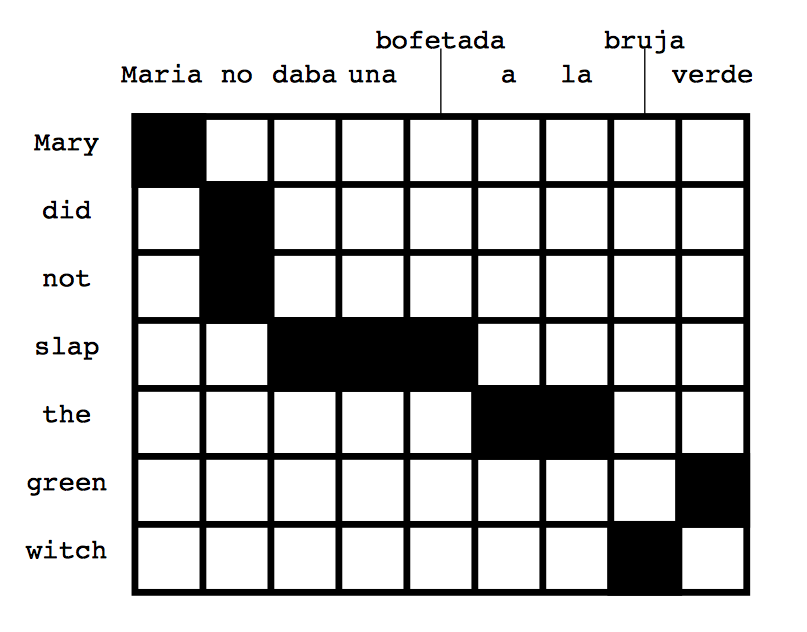
\includegraphics[width=10cm]{files/images/alignmentExample}
\centering
\caption{A sample alignment between a Spanish sentence and English sentence \cite{Koehn2009}}
\label{fig:sample-align}
\end{figure}

It is not easy to find accurate alignments between words of two languages. Specially, for some function words which may or may not have an equivalent word in the other language. Also, it is important that content words in source language are aligned to the corresponding content word in the target language.

Approaches for learning word alignments can be classified into two general categories, as described by \cite{Och2003}, \textit{(a) statistical alignment models}, and \textit{(b) heuristic models}. In this thesis we only focus on \textit{statistical alignment models} and look at various methods in this category. 

In statistical alignment models, we collect statistics from the sentence aligned parallel corpus to generate word alignment models. We are given a source language string $f^J_1 = f_1,..., f_j, ..., f_J$ and a target language string $e^I_1 = e_1, ..., e_i, ..., e_I$. In SMT, we have a translation model $P(f^J_1 | e^I_1)$, which is the translation probability describing the relationship between a source language string and target language string. In this translation model, we introduce a \textit{hidden} alignment $a^J_1$ which describes the mapping between word $f_j$ and $e_i$. This gives us the statistical alignment model as $P(f^J_1, a^J_1 | e^I_1)$. As shown by \cite{Och2003}, the relation between translation model and statistical alignment model is
\begin{eqnarray}
P(f^J_1 | e^I_1) = \sum_{a^J_1} P(f^J_1, a^J_1 | e^I_1)
\end{eqnarray}

To account for the unknown parameters $\theta$ learnt from training data, the statistical alignment model is represented as $p_{\theta}(f^J_1, a^J_1 | e^I_1)$. For each sentence pair $(\mathbf{f_n, e_n})$, for $n = 1, ..., N$, where $N$ is the size of parallel corpus, the alignment is denoted as $\mathbf{a} = a^J_1$. We find the unknown parameters $\theta$ by maximizing the likelihood on the parallel corpus:

\begin{eqnarray}
\hat{\theta} = \arg\!\max_\theta \prod_{n = 1}^{N} \sum_{\mathbf{a}} p_{\theta}(\mathbf{f_n}, \mathbf{a} | \mathbf{e_n})
\end{eqnarray}

To perform the maximization, Expectation Maximization (EM) \cite{Dempster1977} or some variant of it is used. After finding the unknown parameters, the best alignment for a pair of sentences can be calculated as:

\begin{eqnarray}
\hat{a}^J_1 = \arg\!\max_{a^J_1} p_{\hat{\theta}}(f^J_1, a^J_1 | e^I_1)
\end{eqnarray}

Such statistical alignment models are called generative models and are generally created using unsupervised learning techniques. A major drawback of generative models is that incorporating arbitrary features is difficult. For example, if we want to include orthographic similarity between two words, presence of the pair in some dictionary, etc. Another drawback of unsupervised generative models based on EM is that they require large amount of data and processing to converge to a good solution. Discriminative models on the other hand allow us to have arbitrary features. In discriminative models the features do not have to adhere to the independence assumption, that is, features can be dependent on other features. Whereas, generally in generative EM based algorithms, we assume that the features are independent of each other. 

There are various ways to create discriminative models for getting word alignments. Word alignment problem can also be thought of as a maximum weighted matching problem where each pair of words in parallel sentences would be assigned a score depending on how likely they are to be aligned. The word alignment problem can also be considered as a maximum weight bipartite matching problem \cite{Taskar2005}, where nodes correspond to words in the two parallel sentences. Aside from graph matching algorithms, discriminative approaches also use perceptron algorithm \cite{Moore2006}, support vector machines \cite{Cherry2006}, conditional random fields \cite{Blunsom2006} or neural networks \cite{Ayan2005}.

%Apart from the unsupervised learning approach, statistical alignment models can also be created using semi-supervised or supervised learning. In both these techniques, manually annotated alignments of words in parallel sentences are utilized to train the model. In supervised training, the complete training parallel corpus would be manually annotated. In semi-supervised training, only few examples from the complete training corpus are manually annotated and used for training the models. Both these approaches use a held out set of manual alignments to tune the model parameters.
%Even though, supervised learning would allow us to achieve better performance of the model, but getting manually annotated parallel corpus for training is expensive. Semi-supervised learning allows us to reach convergence of the optimization function at a faster rate as compared to unsupervised technique by only using small amount of manually annotated parallel corpus.

\subsection{Translation Model}\label{intro-tm}
In phrase-based SMT, continuous sequence of words (phrases) are the atomic units of translation. The source sentence is first broken down into phrases and each phrase is then translated. To get the translation of source phrase, a phrase table is learnt from the parallel corpora. \cite{Koehn2009} states the following advantages of using phrases as atomic units:
\begin{itemize}
	\item Many-to-many translation can handle non-compositional phrases.
	\item Use of local context in translation.
	\item Longer phrases can be learnt if more data is available.
\end{itemize}

The learning of phrase table can be broken down into three steps:
\begin{itemize}
	\item Get alignments (as described in Section~\ref{section:alignments}) of words from parallel corpora in both directions (bi-directional alignments). To combine the alignments from two runs, there are various heuristics in the literature, but for our work, we use the approach outlined in \cite{Koehn2003} called \textit{grow-diag-final-and}. This heuristic has several steps, in the first step, all \textit{intersection} alignment points are selected. In the \textit{grow-diag} step, neighbouring and diagonally neighbouring alignment points which are in the union but not in the intersection of the two runs are selected. And, in \textit{final-and} step, alignment points which are unaligned and present in the \textit{intersection} are selected . For our work, we use GIZA++ \cite{Och2003} to get the bidirectional alignments.
	
	\item Using the bidirectional alignments from step 1, extract all posible phrase pairs which are consistent with the alignments \cite{Och1999, Koehn2003}. A phrase pair is consistent with the alignments if words within the source phrase are only aligned to words in the target phrase. Table~\ref{table:sample-phrase-pairs} shows all the posible phrase pairs that are consistent with the alignments shown in Fig~\ref{fig:sample-align}.
	
	\item Assign probabilities to phrase pairs using their relative frequencies:
	\begin{eqnarray}
		\phi(\bar{f}|\bar{e}) = \frac{count(\bar{e}, \bar{f})}{\sum_{\bar{f_i}} count(\bar{e}, \bar{f_i})}
	\end{eqnarray}
	Here, $\bar{f}$ is a source phrase and $\bar{e}$ is the target phrase. Along with $\phi(\bar{f} | \bar{e})$, other features like \textit{inverse lexical weighting}, \textit{direct phrase translation probability} and \textit{direct lexical weighting} are also calculated.
\end{itemize}

\begin{table}
	\begin{center}
		\begin{tabular}{|c|c|}
			\hline
			\textbf{Source Phrase} & \textbf{Target Phrase} \\\hline
			Maria & Mary\\
			no & did not \\
			daba una bofeta & slap \\
			a la & the \\
			bruja & witch \\
			verde & green \\
			Maria no & Mary did not \\
			no daba una bofetada & did not slap \\
			daba una bofetada a la & slap the \\
			bruja verde & green witch \\
			Maria no daba una bofetada & Mary did not slap \\
			no daba una bofetada a la & did not slap the \\
			a la burja verde & the green witch \\
			Maria no daba una bofetada a la & Mary did not slap the \\
			daba una bofetada a la burja verde & slap the green witch \\
			no daba una bofetada a la burja verde & did not slap the green witch \\
			Maria no daba una bofetada a la burja verde & Mary did not slap the green witch \\ \hline
		\end{tabular}
		\caption{All possible phrase pairs consistent with the alignments shown in Fig.\ref{fig:sample-align}}
		\label{table:sample-phrase-pairs}		
	\end{center}
\end{table}

At the end of these steps, we get a phrase table containing the bilingual phrase pairs, the alignments within those phrase pairs and feature scores as shown in table~\ref{table:sample-phrase-table-entry}.

\begin{table}
	\begin{center}
		\begin{tabular}{|c|c|c|c|}
			\hline
			\textbf{Source Phrase} & \textbf{Target Phrase} & \textbf{Feature Scores} & \textbf{Alignments}\\\hline
			in europa & in europe & 0.829007 0.207955 0.801493 0.492402 & 0-0 1-1 \\\hline
		\end{tabular}
		\caption{A sample entry in the translation model (phrase table)}
		\label{table:sample-phrase-table-entry}		
	\end{center}
\end{table}


\subsection{Language Model}\label{intro-lm}
Language model is an integral part of an SMT system. The job of a language model is to measure how likely a string of words (sentence) in a language would be uttered by a human speaker, that is, how fluent is the sentence. For example, we have two sentences in English, \textit{"this is a house"} and \textit{"this a house is"}. The language model should tell us that the probability of former sentence should be higher than the latter, that is, $p_{LM}(\textnormal{\textit{this is a house}}) > p_{LM}(\textnormal{\textit{this a house is}})$. From this example, we notice that language models along with telling how fluent a sentence is, they also help in deciding the right order of words. They also help in choosing the right words for translation. For example, $p_{LM}(\textnormal{\textit{I am going home}}) > p_{LM}(\textnormal{\textit{I am going house}})$.

For an SMT system, the language model is trained on large monolingual corpora of the target language. This is because we want to aid the translation system in deciding a good translation for a source sentence. Due to abundance of data available in a single language, the amount of training data used in training the language model is generally orders of magnitude more than the parallel corpora used to train the translation model. 

The state of the art method to train a language model is \textit{n-gram} language modelling. In n-gram language models, we compute the probability of a sentence $W = w_1, w_2, w_3,..., w_n$. The probability of sentence $p(W)$ can be represented as a joint probability of words in the sentence: 
\begin{eqnarray}
	p(W) = p(w_1, w_2, ..., w_n)
\end{eqnarray}

Using chain rule, we can break this down:
\begin{eqnarray}
p(W) = p(w_1)p(w_2|w_1)p(w_3| w_1, w_2)...p(w_n|w_1, w_2, ...,w_{n-1})
\end{eqnarray}

Here, we have broken down the probability of a sentence into probability of words depending on the preceeding words. To be able to calculate these probabilities easily, we limit the history of each word to $m$ words.
\begin{eqnarray}
p(W) = p(w_1)p(w_2|w_1)p(w_3| w_1, w_2)...p(w_n|w_{n-m}, ...,w_{n-2}, w_{n-1})
\end{eqnarray}
This model in which we step through a sequence of words and consider a limited history for each transition is called a \textbf{Markov chain}. Here $m$ is the order of the model. For example, a 3 gram language model would be:
\begin{eqnarray}
p(W) = p(w_1)p(w_2|w_1)p(w_3| w_1, w_2)p(w_4|w_2, w_3)...p(w_n|w_{n-2}, w_{n-1})
\end{eqnarray}

To estimate the probability of the n-grams, we collect the required counts from the monolingual corpora and use maximum likelihood estimation:
\begin{eqnarray}
p(w_3|w_1, w_2) = \frac{count(w_1, w_2, w_3)}{\sum_{w} count(w_1, w_2, w)}
\end{eqnarray}

%Even though we use a large monolingual corpora to train the language model, we still cannot cover every word and it's usage. To tackle the problem of unseen words, the literature describes various smoothing techniques like \textit{add-one smoothing} and \textit{add-\alpha smoothing}. In add-one and add-\alpha smoothing, we add add 1 or some number \alpha > 1 to the count of each word and add the count of vocabulary or \alpha times vocabulary to the normalizer.
Even though we use a large monolingual corpora to train the language model, we still cannot cover every word and it's usage. To tackle the problem of unseen words, the literature describes various smoothing techniques like \textit{add-one smoothing}, \textit{add-$\alpha$ smoothing}, \textit{Good-Turing smoothing} \cite{Good1953}, \textit{Witten-Bell smoothing} \cite{WittenBell1991}, \textit{Kneser-Ney smoothing} \cite{KneserNey1995}, etc. 

\subsection{Decoder}\label{intro-decoder}
\cite{Koehn2003} states the mathematical model for translation as $p(e|f)$. The job of the decoder is to find the translation $e_{best}$ with the highest probability. This can be mathematically formulated as:
\begin{eqnarray}
	e_{best} = {argmax}_e p(e|f)
\end{eqnarray}

\begin{figure}[h]
	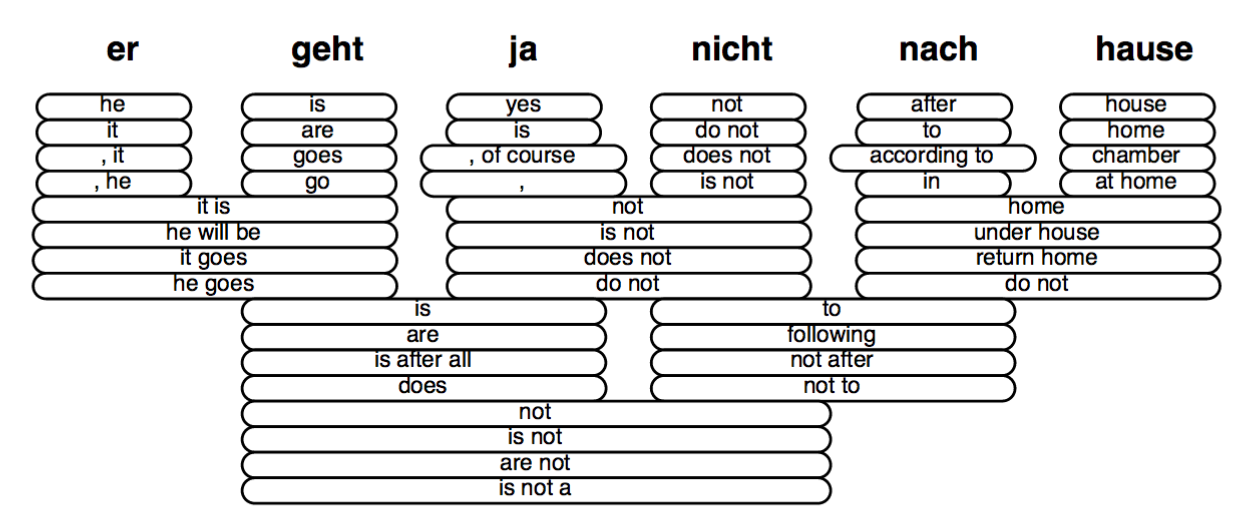
\includegraphics[width=10cm]{files/images/translation-options}
	\centering
	\caption{A sample German source sentence broken into possbile phrases and the top four translation options for each of the source phrase \cite{Koehn2009}}
	\label{fig:sample-translation-options}
\end{figure}

When the decoder proposed by \cite{Koehn2003} has to translate a source sentence, it first breaks the sentence down into the atomic units of phrase-based SMT, that is, phrases as shown in Fig~\ref{fig:sample-translation-options}. The target sentence is then generated left to right in the form of partial translations called hypothesis and it employs a beam search algorithm. The decoder starts with an initial empty hypothesis. A new hypothesis is expanded from an existing hypothesis by selecting the next untranslated source phrase, finding it's possible target phrase from the translation model. The target phrase is appended to the existing target sentence. The hypothesis is then scored using weighted combination of scores from certain feature functions and the source phrase is marked as translated. The final hypothesis in the search tree which has the highest probability is chosen as the best translation for the source sentence as shown in Fig~\ref{fig:sample-search}

\begin{figure}[h]
	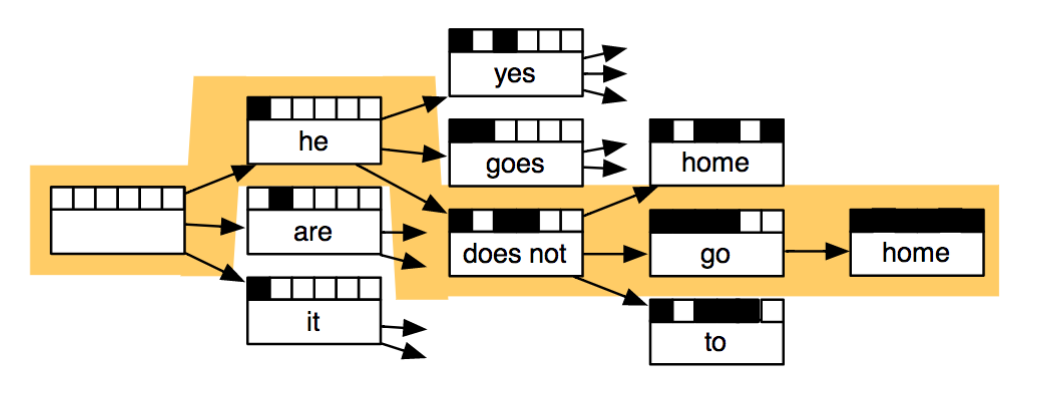
\includegraphics[width=10cm]{files/images/sample-search}
	\centering
	\caption{A sample German source sentence broken into possbile phrases and the top four translation options for each of the source phrase \cite{Koehn2009}}
	\label{fig:sample-search}
\end{figure}

A limitation of this approach is that for each source sentence, exponential number of hypothesis are generated. Searching through these hypothesis is an NP-complete problem \cite{Knight1999}. To tackle this problem, \cite{Koehn2003} proposed using the hypothesis recombination strategy as in \cite{Och2001}. Along with this, hypothesis are also pruned by comparing their current score and the future score proposed by \cite{Koehn2003}. Histogram pruning and threshold pruning proposed by \cite{Koehn2004Pharaoh} are also used to prune the search tree.

We mentioned above that the decoder scores each hypothesis using a weighted combination of scores from various feature functions. We also mentioned above that the decoder uses translation model in it's process. In addition to the feature scores from translation model, the decoder also uses the language model we described earlier, a reordering model which is created using the alignments extracted earlier and various feature functions.

\cite{Koehn2003} proposed a weighted model comprising of the phrase translation model ($\phi(\bar{f}|\bar{e})$), a reordering model ($d$), and language model ($p_{LM}(e)$), which is mathematically formulated as:
\begin{eqnarray}\label{eqn:weighted-model}
	e_{best} = {argmax}_e \prod_{i=1}^{I} \phi(\bar{f}_i|\bar{e}_i)^{\lambda_\phi} d(a_i - b_{i_1} -1)^{\lambda_d} \prod_{i=1}^{|e|}p_{LM}(\textbf{e})^{\lambda_{LM}}
\end{eqnarray}
Here $a_i$ and $b_{i_1}$ are the starting and ending position of the source phrase that was translated to the $i^{th}$ target phrase and ${i-1}^{th}$ target phrase. $\lambda_\phi$, $\lambda_d$ and $\lambda_{LM}$ are the weights for translation model, reordering model and language model respectively. These scores are calculated incrementally for each hypothesis.

Such a weighted model is actually a log-linear model of the form:
\begin{eqnarray}
	p(x) = exp \sum_{i=1}^{n}\lambda_ih_i(x)
\end{eqnarray}

When working with probabilities, it is easier to deal with log values to avoid floating point underflow problems. We can rewrite equation~\ref{eqn:weighted-model} as:
\begin{eqnarray}
	\begin{aligned}
		p(e, a|f)& = exp \big[\lambda_\phi \sum_{i=1}^{I}\log\phi(\bar{f}_i|\bar{e}_i) \\
		& + \lambda_d \sum_{i=1}^{I}\log d(a_i - b_{i-1} -1) \\
		& + \lambda_{LM} \sum_{i}^{|e|} \log p_{LM}(e_1 | e_1 ... e_{i-1})]
	\end{aligned}
\end{eqnarray}

This formulation allows us to add more independent feature functions, that is, feature functions that are independent of other feature functions. In practice, Moses \cite{Koehn2007Moses}, a popular SMT toolkit that we use in our work, uses 15 features which are as follows:
\begin{itemize}
	\item Unknown word penalty
	\item Word penalty (1 feature)
	\item Phrase penalty (1 feature)
	\item Translation model (4 features)
	\item Lexical reordering (6 features)
	\item Distortion (1 feature)
	\item Language model (1 feature)
\end{itemize}

Each of these features have a weight associated with them and it is the job of a tuning algorithm which we will look at in the next section to optimize them.

\subsection{Tuning}
A simple SMT system utilizes number of features during its decoding stage. Each of these features have a weight associated with them. A default value for each of these weights. To understand which of these features are better indicators of a good translation and vice-versa, we need to tune these weights (also called parameters). While tuning, we need to understand the affect of the parameters on translation performance. A popular metric that is used for this is \textbf{B}i\textbf{l}ingual \textbf{E}valuation \textbf{U}nderstudy (BLEU) \cite{Papineni2002}. BLEU compares the output translation with reference translations according to the equation:
\begin{eqnarray}
	BLEU_{score} = BP exp\sum_{i=1}^{n}w_i \log(precision_i)
\end{eqnarray}

Here, BP is called brevity penalty and is formulated as:
\begin{eqnarray}
	BP = \min(1, \frac{output-length}{reference-length})
\end{eqnarray}

$w_i$ are the weights associated with different n-gram precisions. These weights are generally set to 1. Brevity penalty is used to penalize phrases that are much shorter compared to the reference translation. A thing to note is that BLEU score is 0 if any of the n-gram precisions is 0. To calculate \textit{precision}, one simply counts the number of n-grams of system translation which occur in reference translations divided by the total number of n-grams in system translation. The beauty of this precision based metric is that it allows the use of multiple reference translations. Note, reference translations are human generated translations for the source sentence under test.

MT systems can easily over-generate reasonable words, which would result in high precision for sentences like the one in example~\ref{example:bad-bleu-example}. To counter this issue, \textit{modified n-gram precision} exhausts a reference n-gram once it is matched, that is, a reference n-gram once matched cannot be matched again. Fig.~\ref{example:bad-bleu-example} also shows the output of modified n-gram precision.

\begin{figure}[htp]
	\centering
	\begin{boxedminipage}{25em}
		\textbf{System Translation}: \underline{the} the the the the the the.
		
		\textbf{Reference 1}: \underline{The} cat is on \underline{the} mat.
		
		\textbf{Reference 2}: There is a cat on the mat.
		
		\textbf{Modified unigram precision}: $\frac{2}{7}$.
	\end{boxedminipage}
	\caption{An example of modified n-gram precision.}
	\label{example:bad-bleu-example}
\end{figure}

Modified n-gram precision is given as follows:
\begin{eqnarray}
	p_n = \frac{\sum_{C \in SystemTranslation} \sum_{n-gram \in C} Count_{clip}(n-gram)}{\sum_{C\prime \in SystemTranslation} \sum_{n-gram\prime \in C\prime} Count(n-gram\prime)}
\end{eqnarray}

When tuning the parameters of the feature functions, we always use a small parallel corpora that was not used during the training of the models. This small parallel corpora is called the tuning set or dev set. Tuning algorithms can be divided into two main classes:
\begin{itemize}
	\item Batch tuning algorithms: In batch tuning algorithms, the complete tuning set is decoded with some initial weights. Generally an n-best list of decoded output is generated. The tuning algorithm then updates the weights based on the decoder output. The tuning set is again decoded based on the updated weights. This procedure is repeated to optimize the weights until we reach convergence or up to a certain number of iterations. Various such tuning algorithms have been described in the literature, Minimum Error Rate Training (MERT) \cite{Och2003} is the most widely used tuning algorithm. Lattice MERT \cite{Macherey2008} is a variant of MERT that uses lattices instead of n-best list. Pairwise ranked optimization (PRO) \cite{Hopkins2011} works by ranking learning the weight set that ranks the n-best list in the same order as BLEU. Batch MIRA \cite{Cherry2012} is a type of margin based classification algorithm that works in the batch tuning setting.
	\item Online tuning algorithms: Online algorithms work together tightly with the decoder. After decoding each sentence, the tuning algorithm updates the weights before the next sentence is decoded. The MIRA tuning algorithm \cite{Cherry2012} is the most widely used tuning algorithm in this setting.
\end{itemize}

\section{Bi-LMs and why do we need them?}\label{intro-bilm}
In phrase-based SMT, during the decoding process, the decoder decodes a partial hypothesis containing a phrase from the source sentence into the target language. During this process, has very little information from source words outside the current phrase pair. \cite{Stewart2014} states that information from source words outside the current phrase pair is incorporated only indirectly, via target words that are translations of these source words, if the relevant target words are close enough to the current target word to affect the language model scores. To add more information about the source words, \cite{Niehues2011} introduced part-of-speech based \textit{bilingual language models} (Bi-LMs) which was extended by \cite{Stewart2014}. Bilingual language models are generated by aligning each target word in the parallel training corpus with source words to create bitokens. These bitokens are then used to estimate an n-gram language model. Coarse Bi-LMs are Bi-LMs which are estimated by first clustering the bitokens and then estimating the language model. Similarly, coarse LMs are also language models which are estimated by clustering the words and then estimating the language model based on the clustered data. \cite{Niehues2011} generated the Bi-LMs by first replacing the words in the parallel corpus with part-of-speech tags. Using this augmented corpus and alignments, the bitokens were created to estimate the Bi-LMs. Similarly, \cite{Stewart2014} used MKCLS \cite{Och1995} to create word classes. 

In this thesis, we propose a new method of generating Bi-LMs. We create word embeddings and bilingual word embeddings (Chapter~\ref{wordvizChapter} will give an introduction to word embeddings and bilingual word embeddings) of words in our training data. These embeddings are clustered using a spectral clustering algorithm. This allows us to group together words which are semantically similar. These clusters are used to augment the original corpus, hence reducing the vocabulary of the original parallel training corpus. The augmented corporas are used to training Coarse LMs and Bi-LMs (Chapter~\ref{two} explains in detail the steps to create Coarse LMs and Bi-LMs). We call these LMs \& Bi-LMs coarse because they are estimated using data whose vocabulary has been reduced by using certain clusters. In the literature, work has been done to use part-of-speech tags or monolingual clusters of words using Brown clustering algorithm~\cite{Brown1992}. 

In our work we propose three new approaches of creating and using coarse LMs and Bi-LMs to improve statistical machine translation task. We show that our best approach achieves \textbf{+1.4 BLEU points} in the Chinese-English SMT task and two of our approaches achieve an increment in BLEU score by \textbf{0.1} and \textbf{0.4}.

\section{Summary}
In this chapter we introduce the individual steps in training a statistical machine translation system. We then give an introduction to bilingual language models and how they can be helpful in statistical machine translation. In the end we introduce our idea of learning bilingual language models using word embeddings. In Chapter~\ref{wordvizChapter} we will discuss about word embeddings, bilingual word embeddings and a method to judge the best bilingual word embeddings. In Chapter~\ref{two}, we will discuss in detail about bilingual language models. We will also introduce our baseline system and our approaches to develop bilingual language models. Later, in Chapter~\ref{three} we describe our experimental setup and results from our approaches. Finally, in Chapter~\ref{conclusion} we conclude this thesis and introduce ideas that would be natural extensions of our work which we would like to do in the future.
%% Copyright 1998 Pepe Kubon
%%
%% `two.tex' --- 2nd chapter for thes-full.tex, thes-short-tex from
%%               the `csthesis' bundle
%%
%% You are allowed to distribute this file together with all files
%% mentioned in READ.ME.
%%
%% You are not allowed to modify its contents.
%%

%%%%%%%%%%%%%%%%%%%%%%%%%%%%%%%%%%%%%%%%%%%%%%%%%
%
%     Chapter 2   
%
%%%%%%%%%%%%%%%%%%%%%%%%%%%%%%%%%%%%%%%%%%%%%%%%

\chapter{Word Embeddings}
\label{wordvizChapter}

\section{What are word embeddings?}\label{intro-biembedding}
Semantic relations between words denote how two words are related or how close their meanings are. One way to represent this relation is by representing each word as a vector (also called word embeddings) such that, words which are similar, their vectors would lie closer to each other in some $n$ dimension space. Whereas, vectors of dissimilar words would lie far apart. When creating the word embeddings, we assume that words are characterized by the words that surround it, that is the company that the word keeps \cite{Harris1954}. The relation between two vectors (words) is represented by using a displacement vector, that is, a vector between two vectors. The displacement vector can help us find relations like $queen : king :: woman : man$, which would mathematically be denoted as $v_{queen} - v_{king} = v_{woman} - v_{man}$. Here, $v_{i}$ means an $n$-dimension vector of the word $i$. 

Learning word embeddings broadly falls into two categories. \textit{Clustering  based representations}, often use hierarchical clustering methods to group similar words based on their contexts. Brown Clustering \cite{Brown1992} and \cite{Pereira1993} are the two most dominant approaches. Hidden Markov Models can also be used to induce clustering on words \cite{Huang2009}. The problem with clustering approach is that the representations generated are sparse vectors. The reason they are sparse is because the vectors generated would generally be one-hot vectors. Such vectors are contains binary values 0 or 1 where 1 indicates the cluster number to which the word belongs. To reduce the sparsity issues, the other approach is to generate \textit{dense representations} of words. These representations are low dimensional real valued dense vectors. These embeddings can be generated by using latent semantic analysis \cite{Deerwester1990}, canonical correlation analysis \cite{Dhillon2011}, neural-networks \cite{Collobert2008, Huang2012, Mikolov2013a, Mikolov2013b}.

As estimating Bi-LMs required parallel corpora of two languages, it is natural to utilize bilingual word embeddings that denote semantic relations among words across two languages, that is words which are semantically similar in either of the languages are close to each other in some $n$-dimension space. This enables us to understand how close a word in one language would be to another word in the second language. For example, the English word \textit{lake} and Chinese word \textzh{潭} \textit{(deep pond)}, even though they are not direct translations of each other, but due to their semantic similarity, they would be close to each other in some $n$-dimension space. And words which are semantically similar to \textzh{潭} \textit{(deep pond)} and possibly direct translations of \textit{lake} would also be close to each other in that $n$-dimension space. For word embeddings, we measure semantic similarity by measuring the cosine similarity between two word embeddings. It is formally defined as:
\begin{eqnarray}
similarity = cos(\theta) = \frac{\textbf{A}.\textbf{B}}{||\textbf{A}|| ||\textbf{B}||} = \frac{\sum_{i=1}^{n}A_iB_i}{\sqrt{\sum_{i=1}^{n}A_i^2} \sqrt{\sum_{i=1}^{n}B_i^2}}
\end{eqnarray}

Here, $\textbf{A}$ and $\textbf{B}$ are two vectors of size $n$.

Bilingual word embeddings have been created by using various techniques like latent dirichlet allocation and latent semantic analysis \cite{BoydGraber2012, Zhao2006}, canonical correlation analysis \cite{Faruqui2014}, neural-networks \cite{Klementiev12, Zou13, Mikolov2013c, Hermann14, Chandar2014}. In the next section we discuss the reasons for choosing the algorithms to create monolingual and bilingual word embeddings.

\section{Creating Word Embeddings}
As stated in Section~\ref{intro-biembedding}, the underlying idea of most of the methods is based on the concept that the meaning of a word can be determined by the \textit{company that it keeps}. This idea is the underlying method for most of the work done to create monolingual and bilingual word embeddings. For both the embeddings, most of the popular approaches are based on using either canonical correlation analysis~\cite{Dhillon2011, Faruqui2014} and neural networks~\cite{Collobert2008, Huang2012, Klementiev12, Mikolov2013a, Mikolov2013b, Mikolov2013c, Zou13, Hermann14, Chandar2014}. Neural network approaches to create word embeddings have been widely adopted due to the following advantages:
\begin{itemize}
	\item Training the networks can be done using parallel processing and distributed processing.
	\item Graphical processing units (GPU) can be utilized for faster training.
	\item If new data is available for training, the weights of the network can be updated by only using the new data and not the previously used training data. That is, the network does not need to be retrained by using all the previous and new training data. Matrix factorization methods like canonical correlation analysis and latent semantic analysis would require retraining of models using all the data.
	\item They are currently state of the art methods in producing good quality word embeddings.
\end{itemize}

Due to their speed of training and being the state of the art algorithms for training embeddings, we decided to use neural network based approach. For creating monolingual word embeddings we utilize \textbf{Word2Vec}~\cite{Mikolov2013a,Mikolov2013b,Mikolov2013c}, as it is currently state of the art toolkit for creating monolingual word embeddings. We will explain the usage of monolingual embeddings in Chapter~\ref{two}. 

For creating bilingual word embeddings, \cite{Zou13} utilize sentence aligned parallel corpora and their alignments to induce the embeddings whereas \cite{Hermann14} only utilizes a sentence aligned parallel corpora (they state that there is no theoretical dependence on sentence aligned parallel corpora and technically it could also be used with document aligned parallel corpora). As creating alignments is not perfect and they have a small margin of error (the state of the art method to create alignments~\cite{Kirkpatrick2010} for Chinese>English parallel corpus has an alignment error rate of 30\%), using word embeddings that require alignments~\cite{Zou13} would increase the chances of propagating errors. Hence, to keep the possibility of errors in creating alignments and creating bilingual word embedding independent of each other, we use the work of \cite{Hermann14} to create the bilingual word embeddings.

When bilingual word embeddings we need to manually choose multiple hyper-parameters for the algorithms. Varying the hyper-parameters changes the embeddings that are generated. To understand the effects of the hyper-parameters and to choose the ones which give good embeddings we introduce \textbf{WordEmbeddingsViz}\footnote{WordEmbeddingsViz: Tool to visualize bilingual word embeddings \url{https://github.com/anoopsarkar/WordEmbeddingsViz}}, a tool to visualize bilingual word embeddings and to study the effects of different values of hyper-parameters.

In the next section we explain how one can use WordEmbeddingsViz to choose the best embedding parameters.

\section{Visualizing Word Embeddings} \label{WordEmbeddingsViz}

\textbf{WordEmbeddingsViz} enables a user to visualize bilingual word embeddings. The tool uses t-Distributed Stochastic Neighbor Embedding (t-SNE)~\cite{tSNE} to project the embeddings into two dimension space. t-SNE is a non linear dimensionality reduction technique. t-SNE constructs a probability distribution over pairs of objects in high dimension such that similar objects (that is, objects which are close to each other) have a high probability whereas dissimilar objects (objects that are far apart) have a low probability. t-SNE defines a similar probability distribution over pairs of objects in lower dimension and minimizes the Kullback-Leibler divergence between the two distributions. In the higher dimension space, it uses Gaussian distribution to measure the similarity between objects, whereas in lower dimension space, it uses a Student's t-distribution to measure the similarity. This is because, Student's t-distribution has a long tail and it allows dissimilar objects to be modeled far apart.

To use visualize the embeddings, a user will upload the following for each language:
\begin{itemize}
	\item Word Embeddings
	\item Words
	\item Training Corpus (with part-of-speech for one language)
	\item Alignments (optional)
\end{itemize}

\begin{figure}[htbp]
	\begin{center}
		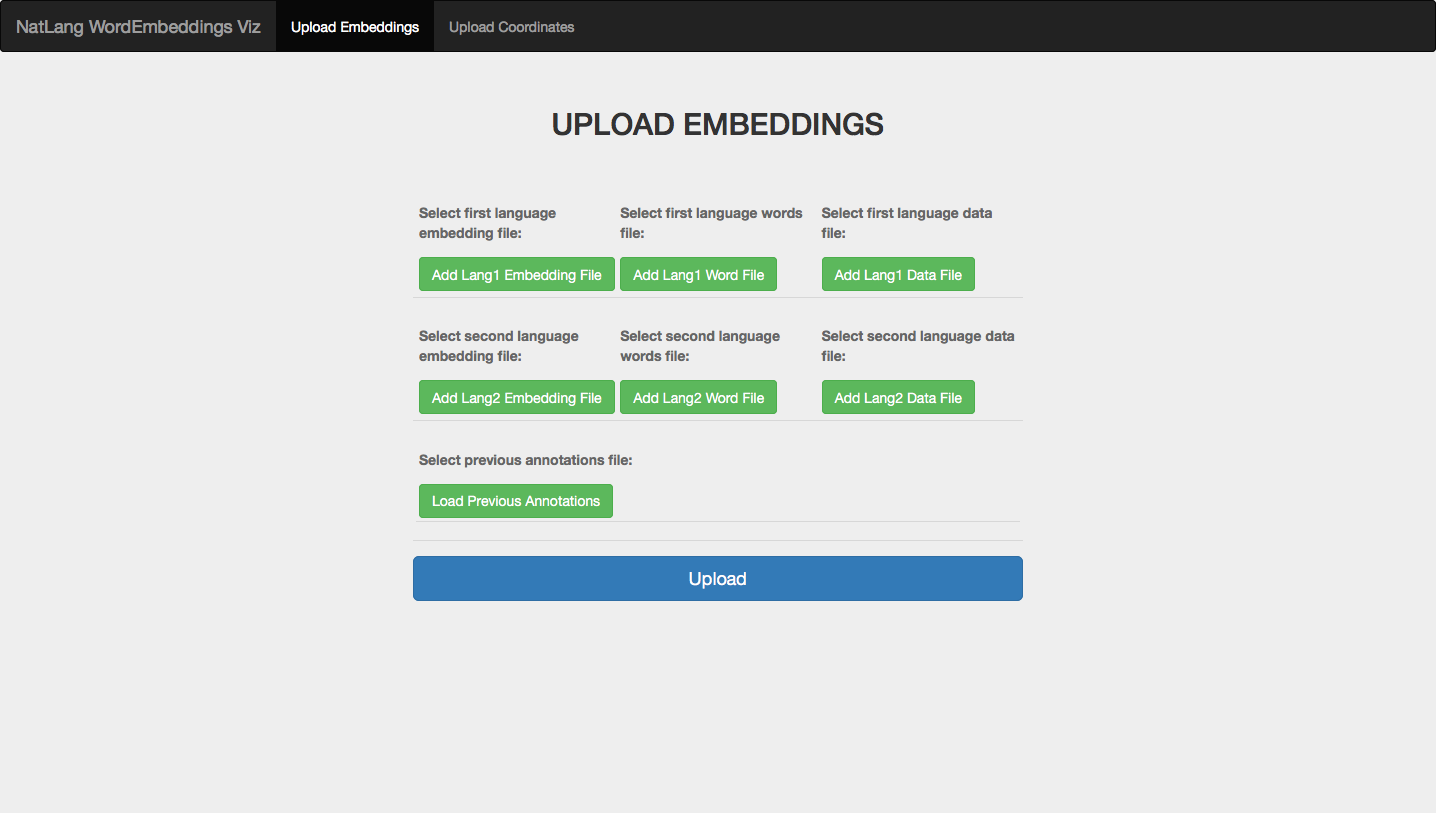
\includegraphics[width=\textwidth]{files/images/viz1}
	\end{center}
	\caption{WordEmbeddingsViz upload screen: Here, the user can upload bilingual word embeddings, word list, training corpus and alignments (optional)}
	\label{fig:viz1}
\end{figure}

Figure~\ref{fig:viz1} shows the upload screen where a user can upload the required data.

We require part-of-speech(POS) for one of the languages as this will be used by the tool to show a list of top 1000 words by their occurance count for \textit{verb, noun, adjective \& adverb} POS tags. For our work, we extracted POS tags for English data using Stanford POS tagger~\cite{POS}.

\textbf{WordEmbeddingsViz} will perform non-linear dimensionality reduction using \textbf{tSNE} on the word embeddings. The dimensions would be reduced to two dimensions. The value of these dimensions for each word would be treated as \textit{x} and \textit{y} coordinates to visualize them as a scatter plot. Figure~\ref{fig:viz2} shows the scatter plot for bilingual word embeddings of Chinese(Zh)-English(En) parallel corpus. The user can then zoom into the scatter plot to look at the word embeddings. The user can also select one of the English words from the sidebar (sidebar shows a list of top 1000 for each of the verbs, nouns, adjectives and adverbs). On selection of a word from the sidebar, that word will be highlighted and the user can then zoom in to look at the neighbouring embeddings. If for any English word, there one or more Chinese words in the neighbourhood that are possible translation of that English word, then the user can align them using the alignment option built into the tool. Figure~\ref{fig:viz3} and Figure~\ref{fig:viz4} shows examples of alignments between English words \textit{broadcast, braodcast \& broadcasting, and, clocks, timepiece \& chiming} along with their Chinese counterparts. The alignments can also be downloaded which can then be utilized for various usecases, such as, using the annotated alignments as information in word alignment algorithms.

\begin{figure}[htbp]
	\begin{center}
		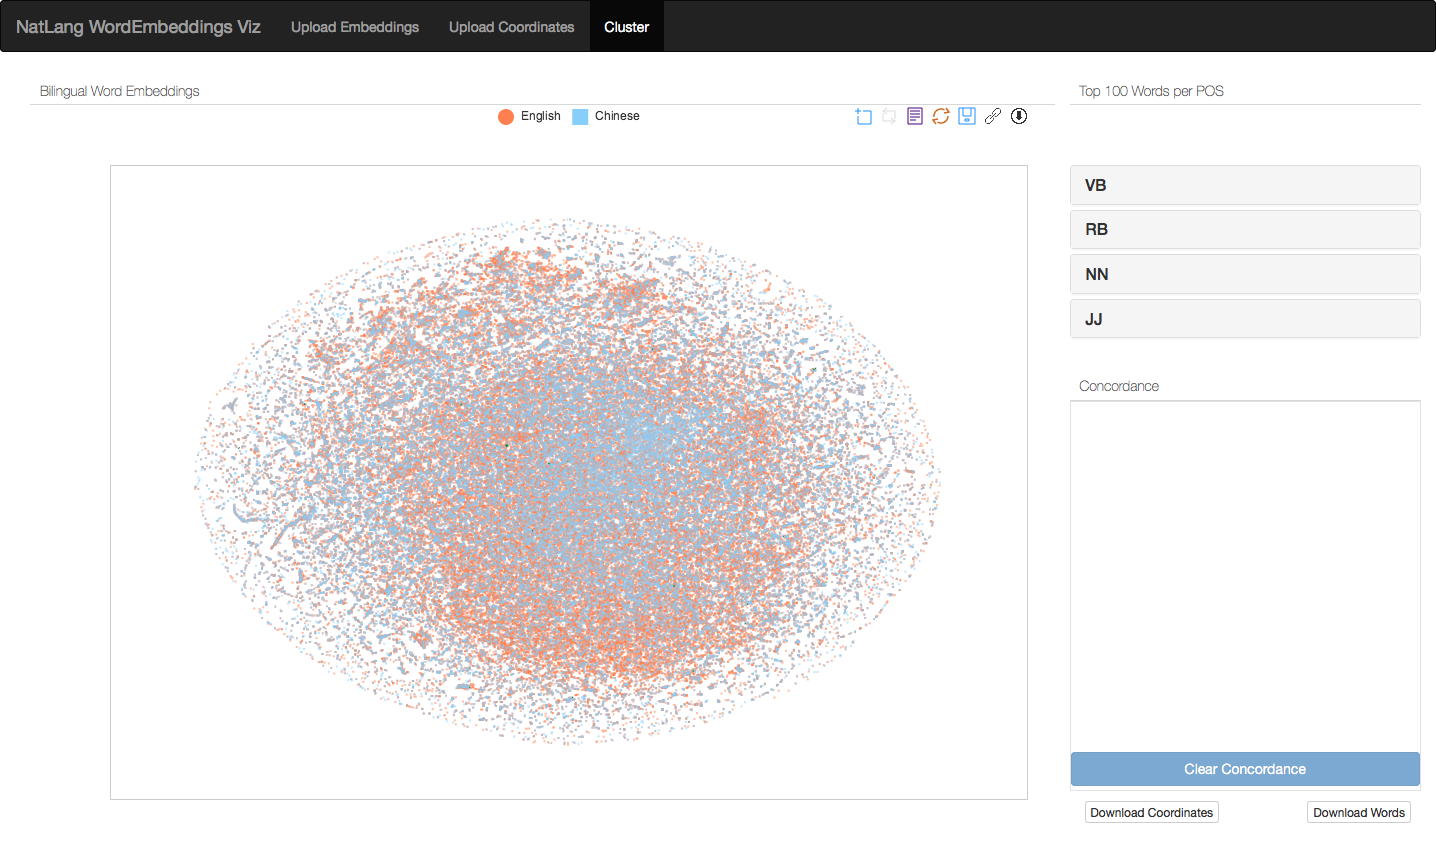
\includegraphics[width=\textwidth]{files/images/viz7}
	\end{center}
	\caption{WordEmbeddingsViz: A scatter plot of word embeddings of Zh-En parallel corpus. Orange squares represent English words and blue circles represent Chinese words.}
	\label{fig:viz2}
\end{figure}

\begin{figure}[htbp]
	\begin{center}
		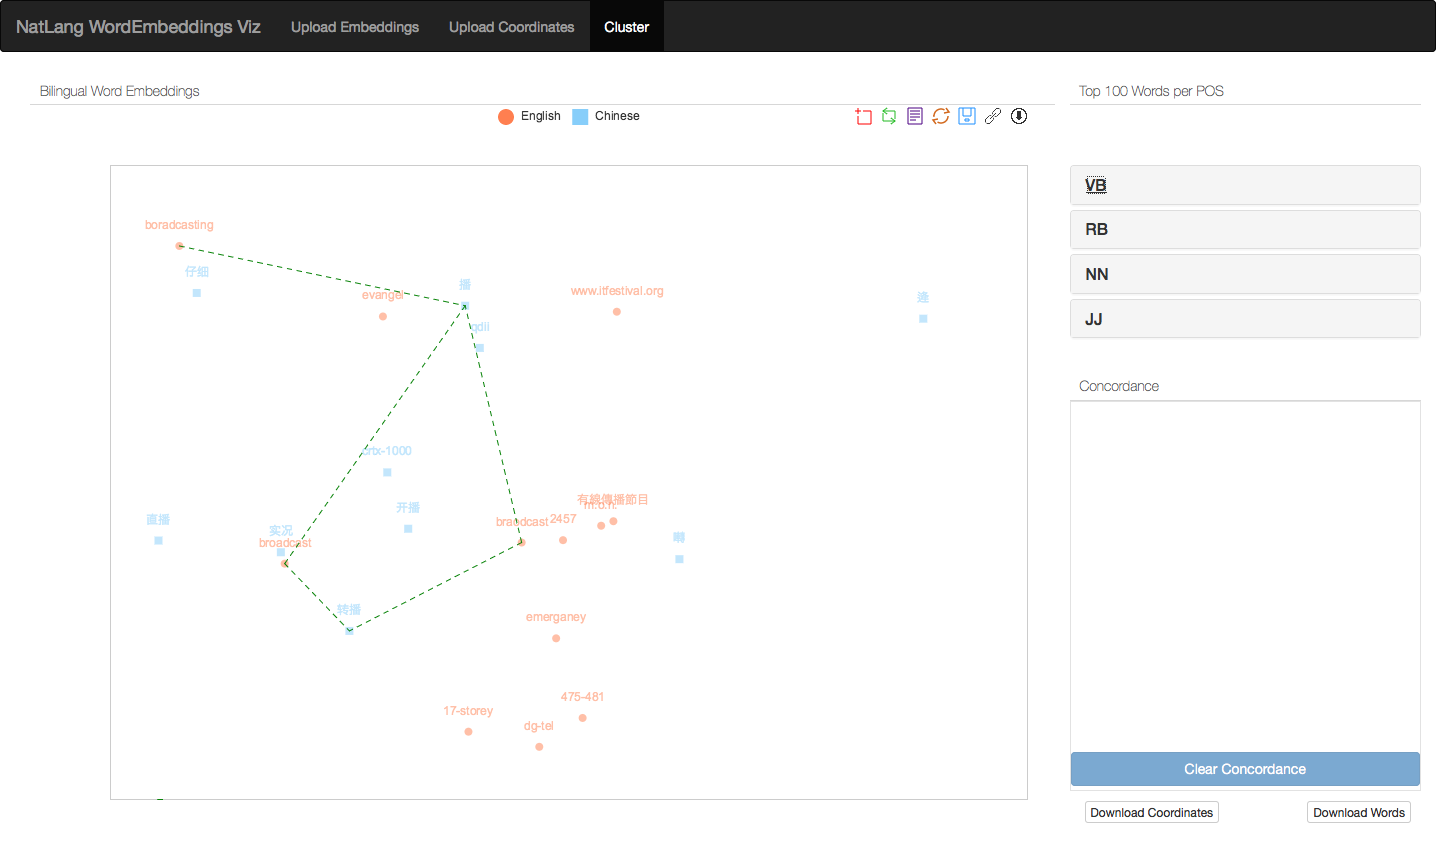
\includegraphics[width=\textwidth]{files/images/viz6}
	\end{center}
	\caption{WordEmbeddingsViz: Alignments of English words \textit{broadcast, braodcast, broadcasting} with their Chinese counterparts.}
	\label{fig:viz3}
\end{figure}

\begin{figure}[htbp]
	\begin{center}
		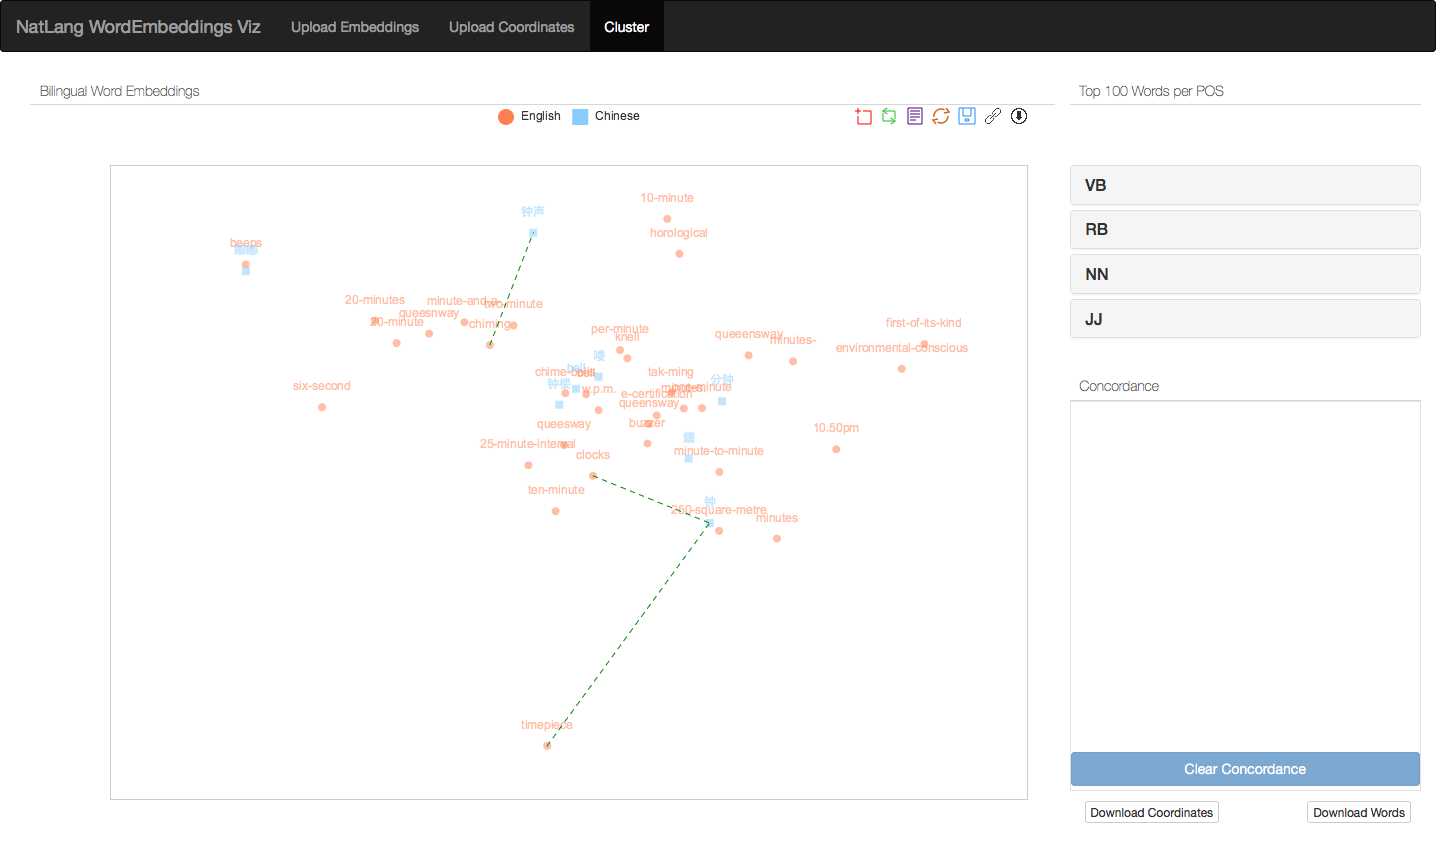
\includegraphics[width=\textwidth]{files/images/viz4}
	\end{center}
	\caption{WordEmbeddingsViz: Alignments of English words \textit{clocks, timepiece \& chiming} with their Chinese counterparts.}
	\label{fig:viz4}
\end{figure}

Using \textbf{WordEmbeddingsViz}, a human annotator can look at bilingual word embeddings generated with different parameters. If the embeddings generated are of good quality then semantically similar words in two languages would lie close to each other in the projected space.

\section{Summary}
In this chapter we introduced word embeddings and bilingual word embeddings. We also release a tool \textbf{WordEmbeddingsViz}, which we developed to judge the bilingual word embeddings. In the next chapter, we will provide an in depth description of bilingual language models and our approach of using word embeddings to model bilingual language models.
%% Copyright 1998 Pepe Kubon
%%
%% `two.tex' --- 2nd chapter for thes-full.tex, thes-short-tex from
%%               the `csthesis' bundle
%%
%% You are allowed to distribute this file together with all files
%% mentioned in READ.ME.
%%
%% You are not allowed to modify its contents.
%%

%%%%%%%%%%%%%%%%%%%%%%%%%%%%%%%%%%%%%%%%%%%%%%%%%
%
%     Chapter 3
%
%%%%%%%%%%%%%%%%%%%%%%%%%%%%%%%%%%%%%%%%%%%%%%%%

\chapter{Bilingual Language Models}
\label{two}

In phrase-based statistical machine translation (SMT), the decoder (Section~\ref{intro-decoder}) breaks down a source sentence into phrases and translates one source phrase at a time. For each source phrase, the decoder uses a translation model (Section~\ref{intro-tm}) to get the corresponding target phrase. To model the target language fluency, it also uses a language model (Section~\ref{intro-lm}). A log-linear combination of these models along with additional features are used to score each hypothesis. The decoder then searches for a path in the search tree which gives the highest hypothesis score for the final translation.

As stated in section~\ref{intro-bilm}, during the decoding process, information from source words outside the current phrase pair in consideration is available indirectly through target words which are translations of these source, if those target words are close enough to affect the language model scores. Due to this, the translation of each source phrase is performed in isolation without significant information from other source words in the sentence. The effect can be seen in the following example:

\begin{figure}[htbp]
	\begin{center}
		Maria no daba una bofetada a la burja verde
	\end{center}
\end{figure}

For this sentence we would get the following phrase segmentations: \textit{Maria no, daba una bofetada a la, bruja verde}. Here, the translation of \textit{Maria no} is not affected by the source words \textit{daba} or \textit{bofetada} or \textit{bruja}. The other possible segmentation could be as shown in Table~\ref{table:sample-phrase-table-entry}. The translation of words \textit{Maria no daba una bofetada a la} can be done using the phrases \textit{Maria no, daba una bofetada a la} or \textit{Maria, no, daba una bofetada, a la}. The decoder cannot make use of the fact that both these options lead to the same translation \textit{Mary did not slap the}. If the first option is chosen, the translation of \textit{no} is affected by \textit{Maria}, but in the second option, \textit{no} is only affected by \textit{Maria} via the language model.

To introduce the effect of source words outside the current phrase pair in consideration, considerable amount of work has been done in the past. In this thesis, we extend the work of \cite{Niehues2011} and \cite{Stewart2014} to create \textit{bilingual language models (Bi-LMs)} that will be used as additional features to the decoder.

\section{What are Bilingual Language Models?}
Bi-LMs are n-gram language models which are trained on bitokens instead of simple word tokens as done for standard language models (Section~\ref{intro-lm}). Bitokens are generated using the source and target sentences from the parallel corpora and their alignments. To understand what bitokens are, let us look at two parallel sentences shown in Fig.~\ref{fig:bitoken-sentences}:

\begin{figure}[htbp]
	\begin{center}
		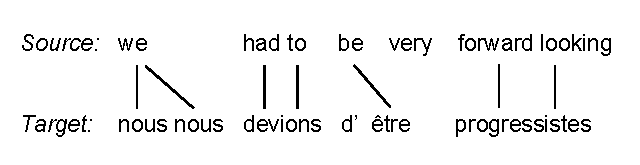
\includegraphics[width=10cm]{files/images/bitoken-example}
	\end{center}
	\caption{Source and target sentences with their alignments for creating bitokens \cite{Stewart2014}}
	\label{fig:bitoken-sentences}
\end{figure}

Using the parallel sentences and their alignments shown above we will create a bitoken sequence. When creating hte bitokens, we want to make sure that all the target words are used. In the exmample above, the source word \textit{we} is aligned to target words \textit{nous nous}. We will replicate \textit{we} twice and align both \textit{nous} with both the \textit{we} to create the bitokens \textit{we-nous} and \textit{we-nous}. Next we have the source words \textit{had to} aligned to \textit{devions}. We will join \textit{had} and \textit{to} to create a single token \textit{had\_to} and align that to \textit{devions} to get \textit{had\_to-devions}. Since, the target word \textit{d'} is not aligned to any source word, we align it to \textit{NULL} and create a bitoken \textit{NULL-d'}. For the source word \textit{very}, as it is not aligned to any target word, it is dropped. Similarly, we also get the bitoken \textit{forward\_looking-progressistes}. The final bitokens are shown in Fig.~\ref{fig:bitokens}:

\begin{figure}[htbp]
	\begin{center}
		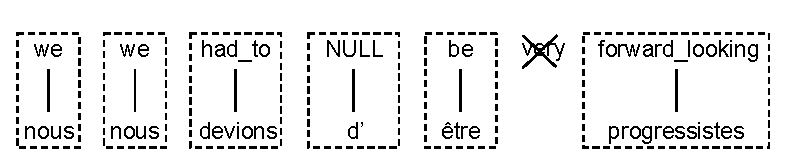
\includegraphics[width=10cm]{files/images/bitoken-example2}
	\end{center}
	\caption{Bitokens created from the parallel sentences and their alignments shown in Fig.~\ref{fig:bitoken-sentences}}
	\label{fig:bitokens}
\end{figure}

More formaly, given a pair of sentences $e_1^I = e_1 ... e_I$, $f_1^J = f_1 ... f_J$ and alignments $A=\{(i, j)\}$, the bitokens are:
\begin{eqnarray}
	b_j = \{f_j\} \cup \{e_i | (i, j) \in A\}
\end{eqnarray}

This makes sure that the number of bitokens $b_j$ are equal to the number of target words. These bitoken sequences can then be used to create a language model called bilingual language model, formalized as follows:

\begin{eqnarray}\label{eqn:bitoken}
p(e_1^I, f_1^J, A) = \prod_{j=1}^J P(b_j | b_{j-1}...b_{j-n})
\end{eqnarray}

The advantage of using Bi-LMs is that they can be used in phrase-based SMT as additional features in the log linear model. When the decoder scores each hypothesis using scores from translation and language model, it can easily incorporate the probability from Eqn.~\ref{eqn:bitoken}. Even though, Bi-LMs are language models, but they act more as translation models as they do not model the fluency of target language but model the translation of source words.

In Bi-LMs the bitoken vocabulary size increases by many folds compared to the vocabulary size of target words. For example, as shown by \cite{Stewart2014}, the target word \textit{être} might be split into multiple bitokens: \textit{be-être}, \textit{being-être} and \textit{to\_be-être}. This large vocabulary also leads to an increase in the sparsity in data for language modelling. Table~\ref{table:vocab-comparison} shows the number of bitokens compared to the number of target words in our corpus. We will explain in detail about our data and alignments used to create the bitokens in Chapter~\ref{three}. 

\begin{table}
	\begin{center}
		\begin{tabular}{|c|c|}
			\hline
			\textbf{Number of Target Words} & \textbf{Number of Bitokens}\\\hline
			152318 & 3827728\\\hline
		\end{tabular}
		\caption{Number of target words vs number of bitokens in our data}
		\label{table:vocab-comparison}		
	\end{center}
\end{table}

%In the next section we discuss the method adopted to handle the large bitoken vocabulary.

%\section{Tackling Sparsity in Language Models}
%In the previous section we see that bitokens have a larger vocabulary than the target language vocabulary of the training data. 
To tackle the problem of large vocabulary and sparsity, \cite{Niehues2011} introduced coarse Bi-LMs. When training LMs and Bi-LMs, if the words are replaced by some word class to reduce the vocabulary size, they are then called \textit{Coarse LMs/Bi-LMs}. When creating Bi-LMs, \cite{Niehues2011} replaced both the source and target words in their Arabic>English SMT with the corresponding Part-of-Speech tags. \cite{Stewart2014} extended this idea and replaced both source and target words with cluster ids generated using \textbf{mkcls} \cite{Och1995}. \cite{Stewart2014} not only clustered the initial source and target words, but also experimented with clustering the bitokens too. Figure~\ref{fig:bitokens-clusters} shows the 3 ways of creating bitoken sequences for Bi-LMs:
\begin{itemize}
	\item Word Clustering: Create bitoken sequences with only source and target word cluster ids. The bitokens are then used to create Bi-LMs.
	\item Bitoken Clustering 1: Create bitokens without clustering source and target words. Cluster the bitokens and then use the bitoken sequences augmented with bitoken cluster ids to create Bi-LMs.
	\item Bitoken Clustering 2: Create bitoken sequences with source and target word cluster ids. Cluster the bitoken sequences and then use the bitoken sequences with bitoken cluster ids to create Bi-LMs.
\end{itemize}

\begin{figure}[htbp]
	\begin{center}
		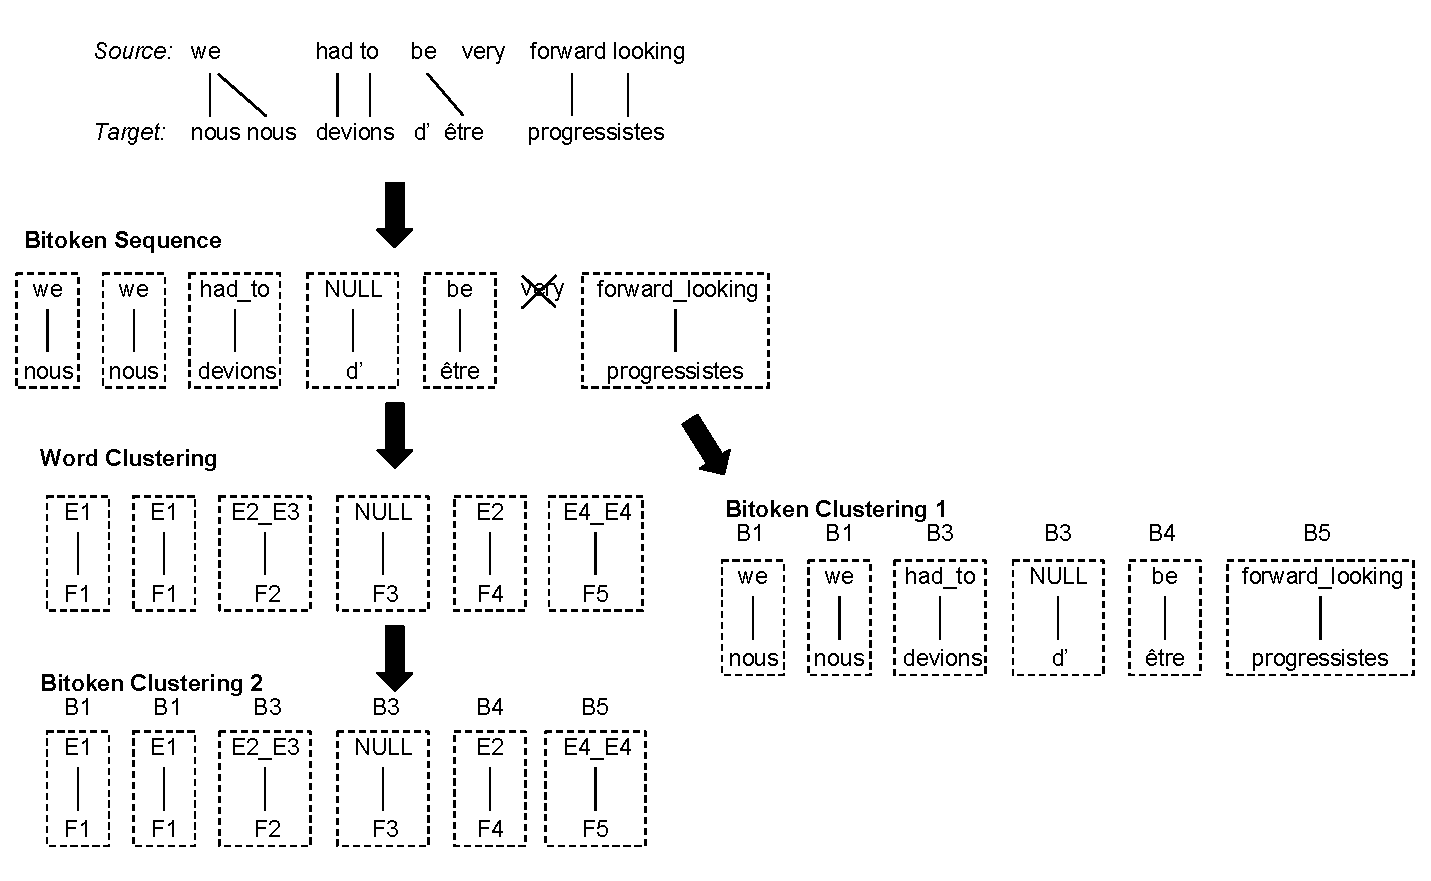
\includegraphics[width=15cm]{files/images/bitoken-example3}
	\end{center}
	\caption{Creating bitokens, word clusters and bitoken clusters \cite{Stewart2014}}
	\label{fig:bitokens-clusters}
\end{figure}

\cite{Ammar2013,Bisazza2014} showed that coarse LMs along with the standard LM are particularly effective for morpholigically rich languages. Motivated by this, \cite{Stewart2014} used a combination of coarse LMs and coarse Bi-LMs in their experiments, which are as follows:
\begin{itemize}
	\item Coarse LM created by augmenting the target language corpus with word cluster ids of size 100. (Coarse LM $100_{tgt}$)
	\item Coarse LM created by augmenting the target language corpus with word cluster ids of size 100. (Coarse LM $1600_{tgt}$)
	\item Augment the source and target language corpus with word cluster ids of size 400 and 400 respectively. This augmented corpus along with their alignments was used to create bitoken sequences. These bitoken sequences were used to create the following two coarse Bi-LMs:
	\begin{itemize}
		\item Use the bitoken sequences to train a coarse Bi-LM. (Coarse Bi-LM $(400_{src},\ 400_{tgt})$)
		\item Cluster the bitoken sequences to get bitoken cluster ids of size 400. Augment the corpus using these bitoken cluster ids to create clustered bitoken sequences. Use these sequences to train a coarse Bi-LM. (Coarse Bi-LM $400_{bi}(400_{src},\ 400_{tgt})$).
	\end{itemize}
\end{itemize}

Figure~\ref{fig:baseline} shows in detail the steps taken by \cite{Stewart2014} to create coarse LM and coarse Bi-LMs. The four coarse LMs and Bi-LMs are then used as additional features in phrase-based SMT. We use this system as a baseline to compare with our results. For our work, we used Moses decoder \cite{Koehn2007Moses} and added additional stateful feature functions to use these coarse LMs and Bi-LMs. Also, to create the LMs and Bi-LMs we used \textbf{SRILM}~\cite{Srilm}.

\begin{figure}[htbp]
	\begin{center}
		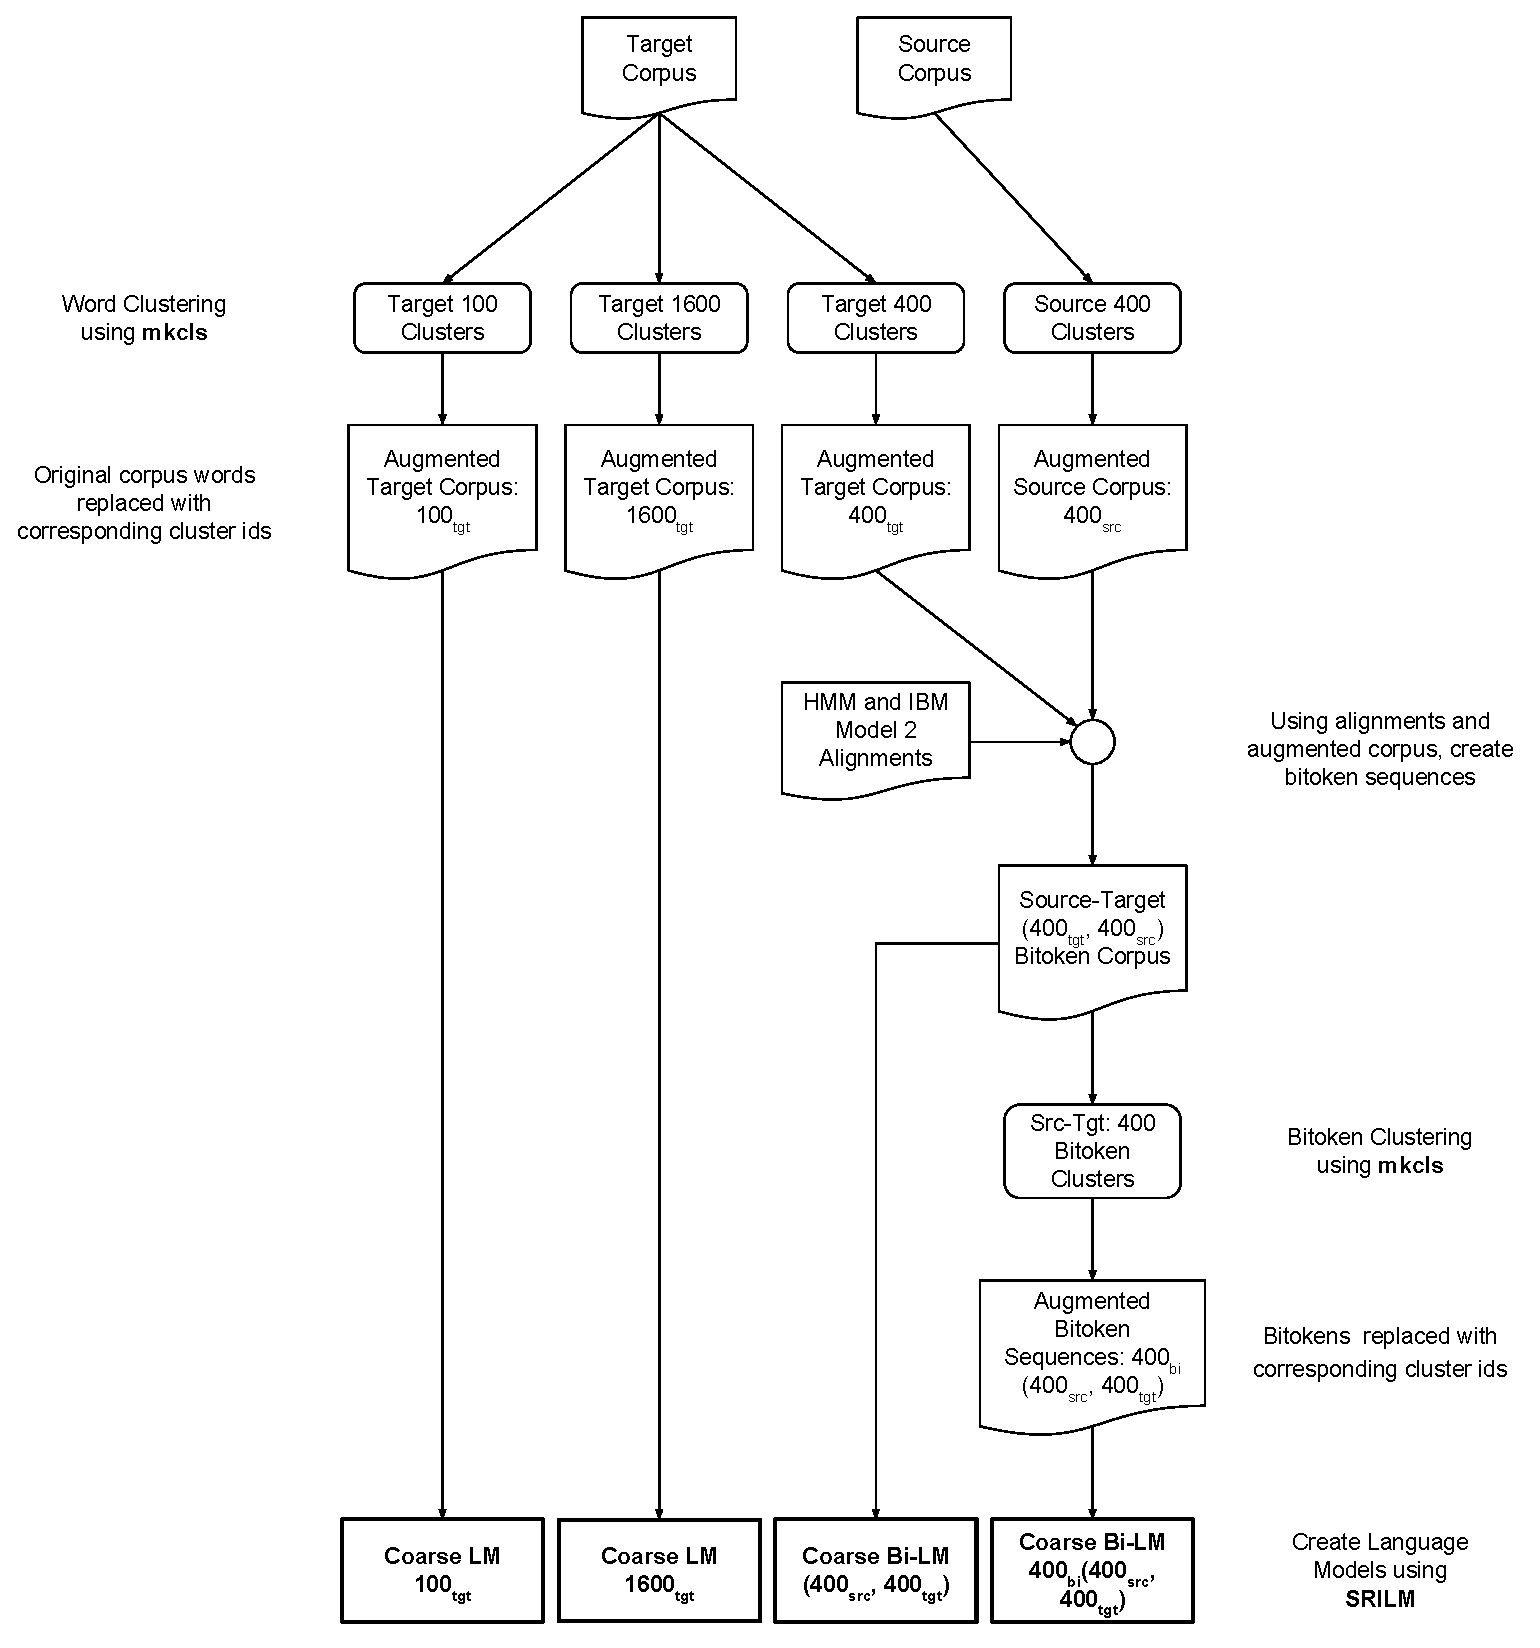
\includegraphics[width=\textwidth]{files/images/baseline}
	\end{center}
	\caption{Creating coarse LMs and coarse Bi-LMs \cite{Stewart2014}}
	\label{fig:baseline}
\end{figure}

In this thesis we extend the work of \cite{Stewart2014} to improve coarse LMs and Bi-LMs. In the next section, we describe in detail the contribution of this thesis, that is, using word embeddings to improve coarse LMs and Bi-LMs.

\section{Bi-LMs using Word Embeddings}
\textbf{mkcls}~\cite{Och1995} is one of the most widely used word clustering toolkit. Motivated by Brown Clustering \cite{Brown1992}, \textbf{mkcls}\footnote{Understanding \textbf{mkcls} by Dr. Chris Dyer: \url{http://statmt.blogspot.ca/2014/07/understanding-mkcls.html}} implements an ensemble of optimzers and merges their results to cluster words into the provided number of classes. \textbf{mkcls} can only cluster monolingual corpus and it performes strongly in that aspect \cite{Blunsom2011}.

The main goal of Bi-LMs is to add more information about source words that are not in the current phrase pair. But current state of the art coarse Bi-LMs only depend on alignments and monolingual word clusters to add more information about source words. For example, the English word \textit{lake} and Chinese word \textzh{潭} \textit{(deep pond)}, which are not direct translations of each other, won't be captured by alignments and hence won't be influencing the coarse Bi-LMs until unless \textbf{mkcls} assigns \textzh{潭} and another Chinese word which is a direct translation of \textit{lake} to the same cluster. To increase the probability that words in Chinese which are semantically similar to \textit{lake} and possibly direct translations get clubbed together in a cluster, we utilize bilingual word embeddings to create the coarse Bi-LMs.

\subsection{Using Word Embeddings to create Bi-LMs}\label{approaches}
In Chapter~\ref{wordvizChapter}, we mention that we utilize \cite{Hermann14} to create bilingual word embeddings for the words in our sentence aligned parallel corpus. To create coarse LMs and Bi-LMs, as done by \cite{Stewart2014}, we need to cluster these embeddings. As mentioned earlier, in our baseline system, we used \textbf{mkcls} to cluster the words in our parallel corpus. To cluster word embeddings, we used \textbf{greedo}~\cite{Stratos2014}, a bottom-up hierarchical clustering algorithm for clustering low-dimensional representation of words under the \cite{Brown1992} model. \cite{Stratos2014} show that the clusters created by \textbf{greedo} recovers clusters which are of comparable quality to the algorithm of \cite{Brown1992}. Using \textbf{greedo} gives us the opportunity to compare our approach to the baseline system without any modifications to the number of clusters because \textbf{mkcls} is also creates Brown clusters.

To use the embeddings and their clusters for creating coarse LMs and coarse Bi-LMs, we propose three approaches.

\subsubsection{Approach 1}\label{approach1}
Once we create the bilingual word embeddings, we can then use them to create the LMs. Figure~\ref{fig:idea1} shows the steps that we took to create our coarse LMs and Bi-LMs. As we did in the baseline, we had clustered the corpora using \textbf{mkcls}, but now we cluster the bilingual word embeddings using \textbf{greedo} to create the following clusters:

\begin{itemize}
	\item Cluster the target language embeddings into clusters of size 100, 400 and 1600.
	\item Cluster the source language embeddings into cluster of size 400. 
\end{itemize}

Using the target language embedding clusters of size 100 and 1600, we augment the target language corpus by replacing the words with their cluster ids. This augmented data is then used to create coarse LMs \textit{Coarse LM $100_{tgt}$} and \textit{Coarse LM $1600_{tgt}$} correspondingly using the language modelling toolkit \textbf{SRILM}.

Using the clusters of size 400 for Target and Source, we augment the parallel corpus by replacing the words with their cluster ids. Using the alignments between the source and target words on the original parallel corpus, we create bitoken sequences. \textit{Coarse Bi-LM $(400_{src},\ 400_{tgt})$} is estimated using the bitoken sequences. The bitoken sequences are further clustered to reduce the vocabulary using \textbf{mkcls}. The size of the cluster in this case is also 400 as done in the baseline system. The bitokens in bitoken sequences are replaced with the new cluster ids. This augmented bitoken sequences is finally used to estimate \textit{Coarse Bi-LM $400_{bi}(400_{src},\ 400_{tgt})$}.

\begin{figure}[htbp]
	\begin{center}
		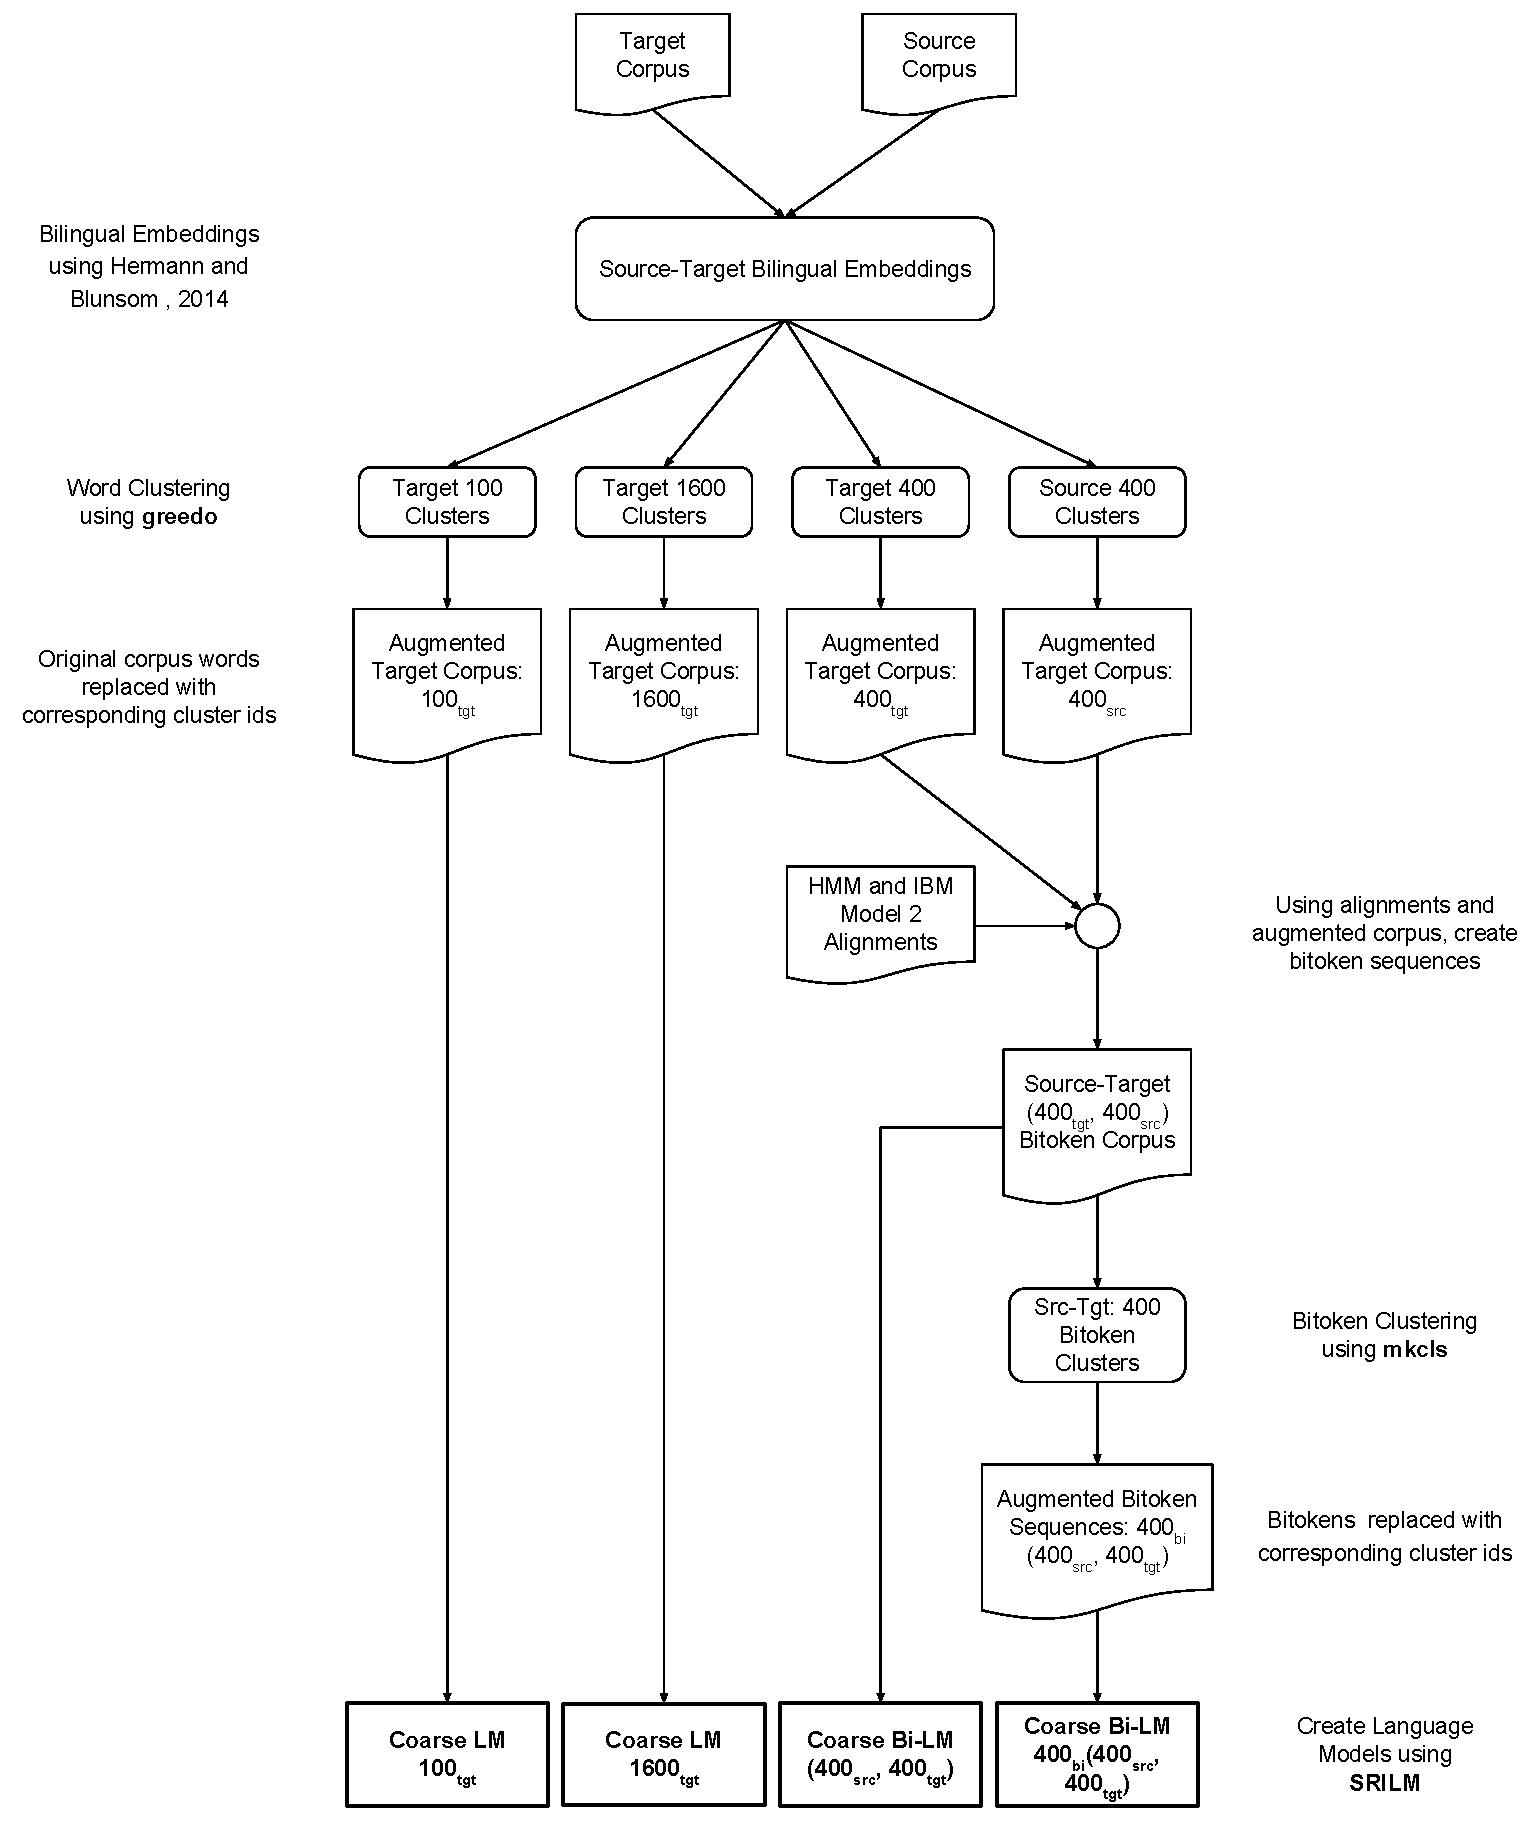
\includegraphics[width=\textwidth]{files/images/idea1}
	\end{center}
	\caption{Approach 1 for creating Coarse LMs and Coarse Bi-LMs}
	\label{fig:idea1}
\end{figure}

\subsubsection{Approach 2}\label{approach2}
Figure~\ref{fig:idea2} shows our second idea to create coarse LMs and Bi-LMs. Based on Approach 1~\ref{approach1}, we first create bilingual word embeddings using \cite{Hermann14} for the sentence aligned parallel corpus used for training the SMT system. The bilingual word embeddings are clustered using \textbf{greedo} to create the same clusters as in Approach 1, which are:
\begin{itemize}
	\item Target language word embedding clusters of size 100, 400 and 1600.
	\item Source language word embeddings cluster of size 400.
\end{itemize}

The clusters are then used to augment the source and target language corpus by replacing the words with their cluster ids. Augmented target language corpus \textit{$100_{tgt}$} and \textit{$1600_{tgt}$} are used to estimate coarse LMs \textit{Coarse LM $100_{tgt}$} and \textit{Coarse LM $1600_{tgt}$}. Augmented corporas \textit{$400_{tgt}$} and \textit{$400_{src}$} along with bidirectional word alignments of the original corpora are used to create bitoken sequences \textit{($400_{src},\ 400_{tgt}$)}. \textit{Coarse Bi-LM $(400_{src},\ 400_{tgt})$} is estimated using the bitoken sequences.

Using \textbf{word2vec}~\cite{Mikolov2013a}, we create bitoken embeddings for bitoken sequence corpus \textit{$(400_{src}, 400_{tgt})$}. As in our baseline system (Figure~\ref{fig:baseline}) and approach 1 (Figure~\ref{fig:idea1}) we had clustered the bitoken sequences using \textbf{mkcls}, we again create clusters of size \textit{400} by clustering the bitoken embeddings using \textbf{greedo}. The bitokens in bitoken sequence corpus \textit{$(400_{src},\ 400_{tgt})$} are replaced with their cluster ids from \textbf{greedo}. The augmented bitoken sequences \textit{$400_{bi}(400_{src},\ 400_{tgt})$} are used to estimate coarse Bi-LM \textit{Coarse Bi-LM $400_{bi}(400_{src},\ 400_{tgt})$} using \textbf{SRILM}.

\begin{figure}[htbp]
	\begin{center}
		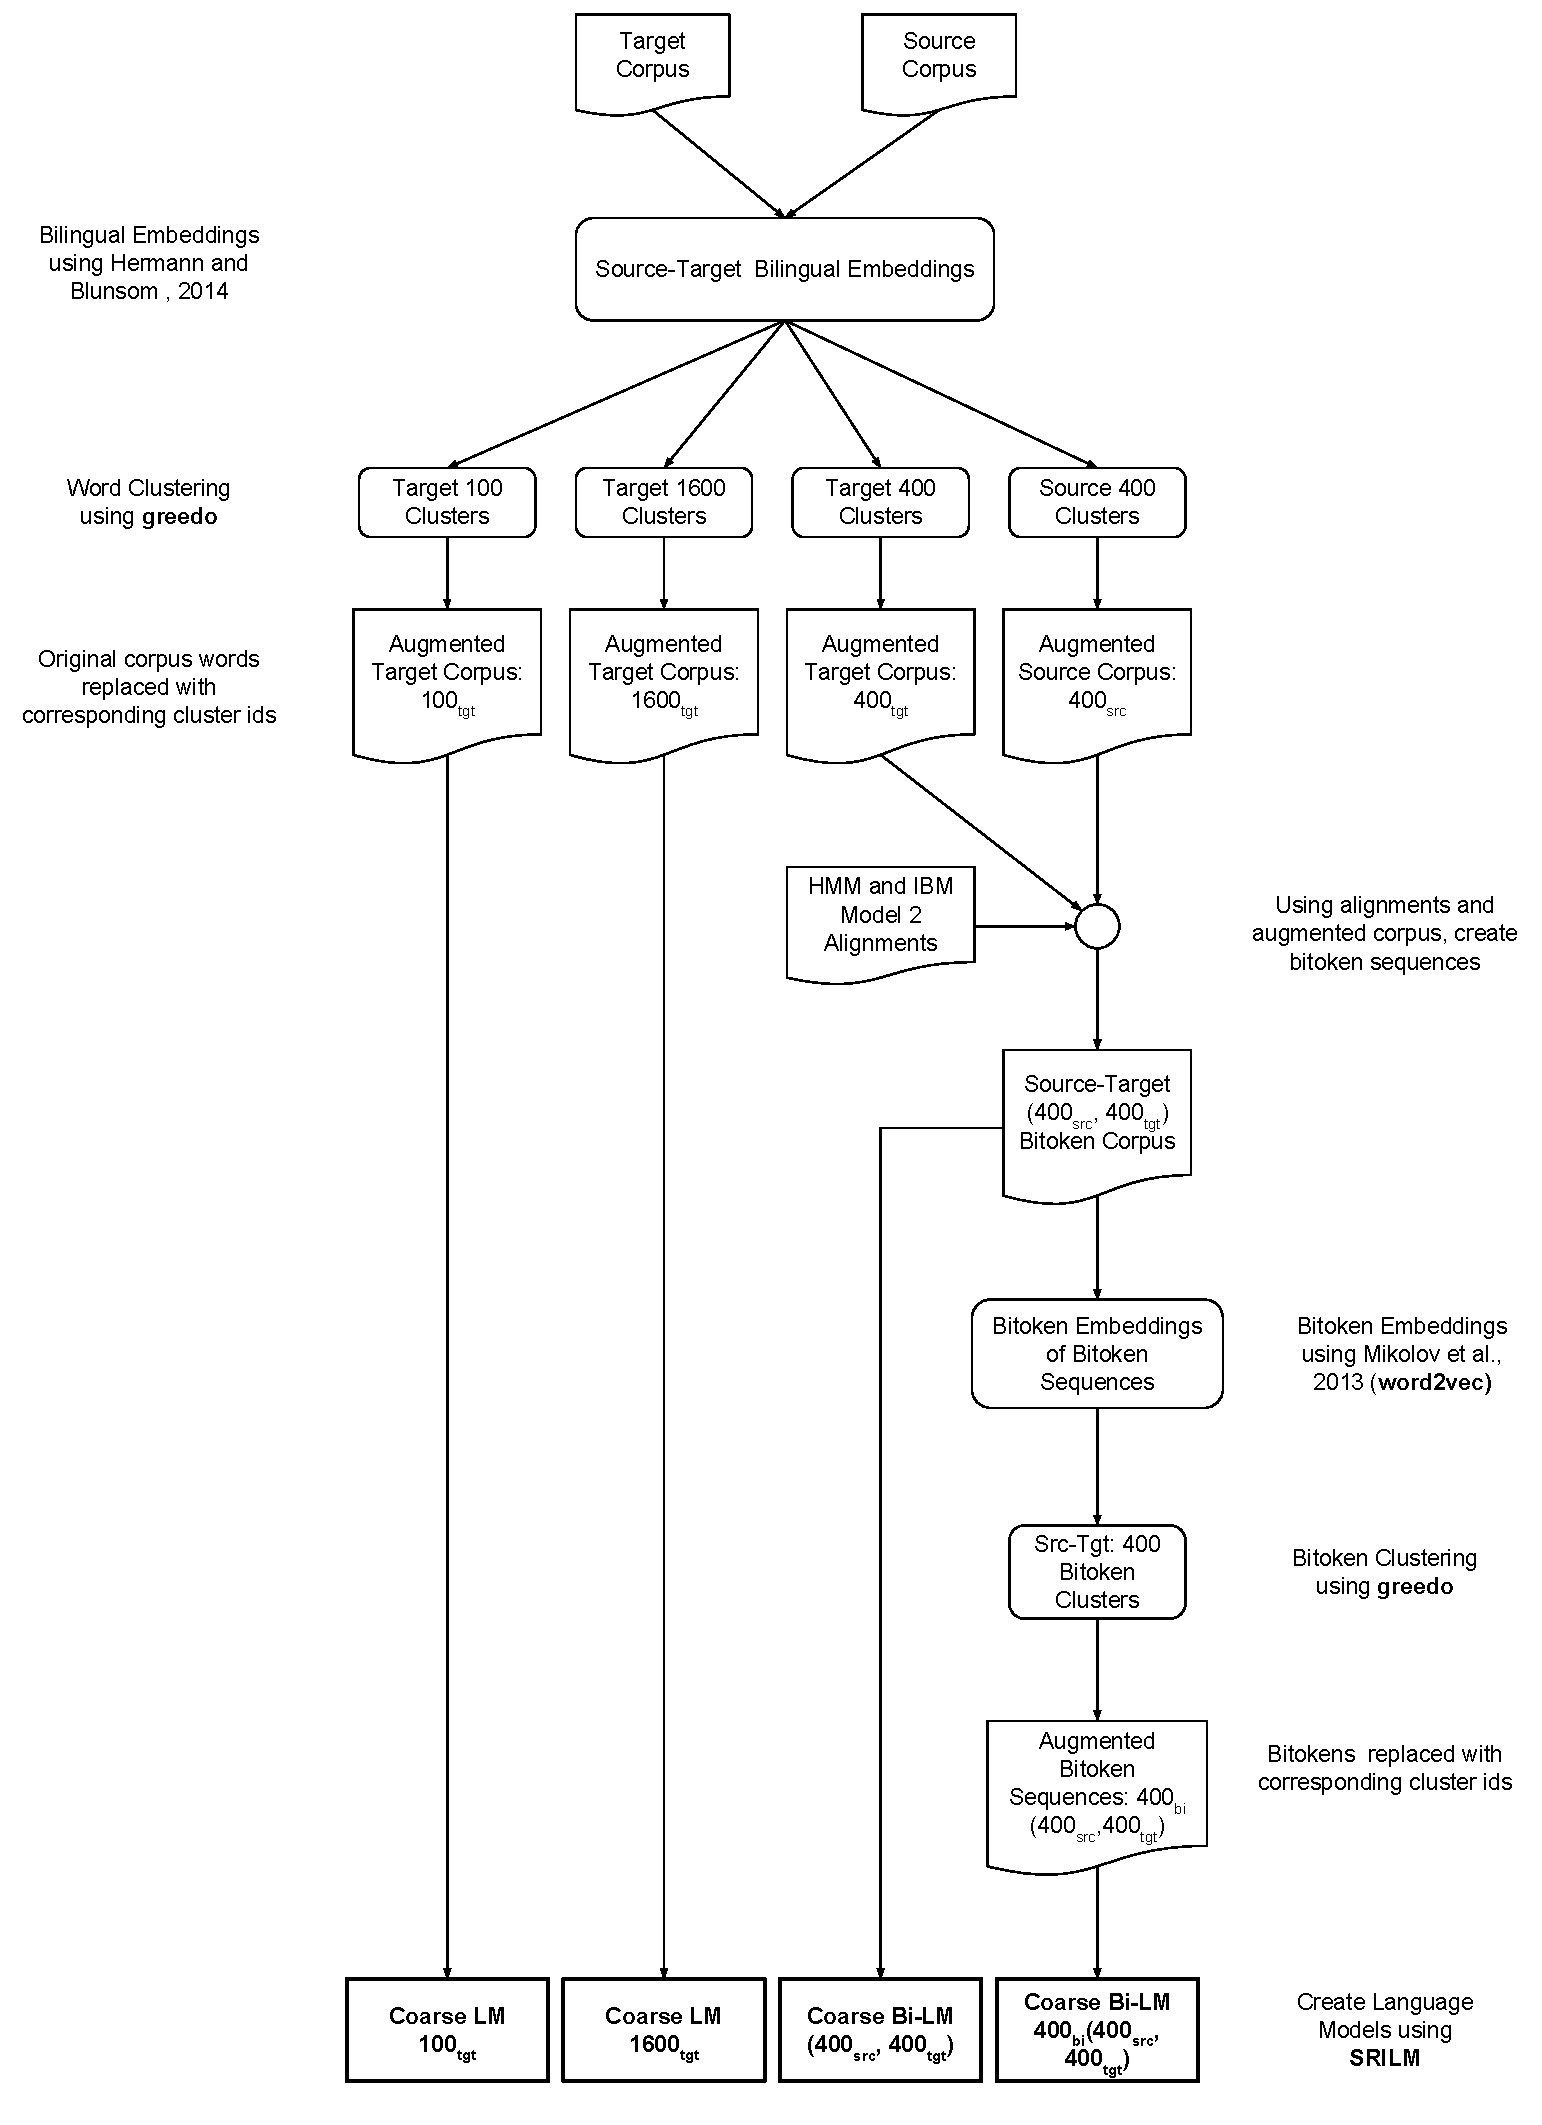
\includegraphics[width=\textwidth]{files/images/idea2}
	\end{center}
	\caption{Approach 2 for creating Coarse LMs and Coarse Bi-LMs}
	\label{fig:idea2}
\end{figure}

\subsubsection{Approach 3}\label{approach3}
In approach 3 (shown in Figure~\ref{fig:idea3}), we estimate the coarse LMs \textit{Coarse LM $100_{tgt}$} and \textit{Coarse LM $1600_{tgt}$} using the same procedure as in approach 1 (\ref{approach1}) and approach 2 (\ref{approach2}).

To create coarse Bi-LM, we first create bitoken sequences using the original sentence aligned parallel corpus along with their alignments. Note, we did not cluster the data before creating the bitoken sequences. Using \textbf{word2vec}, we create bitoken embeddings from the bitoken sequences. The bitoken embeddings are clustered using \textbf{greedo}, with the number of clusters being 400, as done in previous approaches. The bitokens in bitoken sequences are replaced with their corresponding cluster ids to create an augmented corpus \textit{$400_{bi}(|V|_{src},\ |V|_{tgt}$)}. Here \textit{$|V|_{tgt}$} denotes the vocabulary size of target language corpus and \textit{$|V|_{src}$} is the vocabulary size of source language corpus. \textbf{SRILM} is then utilized to estimate \textit{Coarse Bi-LM $400_{bi}(|V|_{src},\ |V|_{tgt})$} using the augmented bitoken corpus \textit{$400_{bi}(|V|_{src},\ |V|_{tgt})$}.

As compared to baseline, approach 1 and approach 2, approach 3 only has one coarse Bi-LM while others have two.

\begin{figure}[htbp]
	\begin{center}
		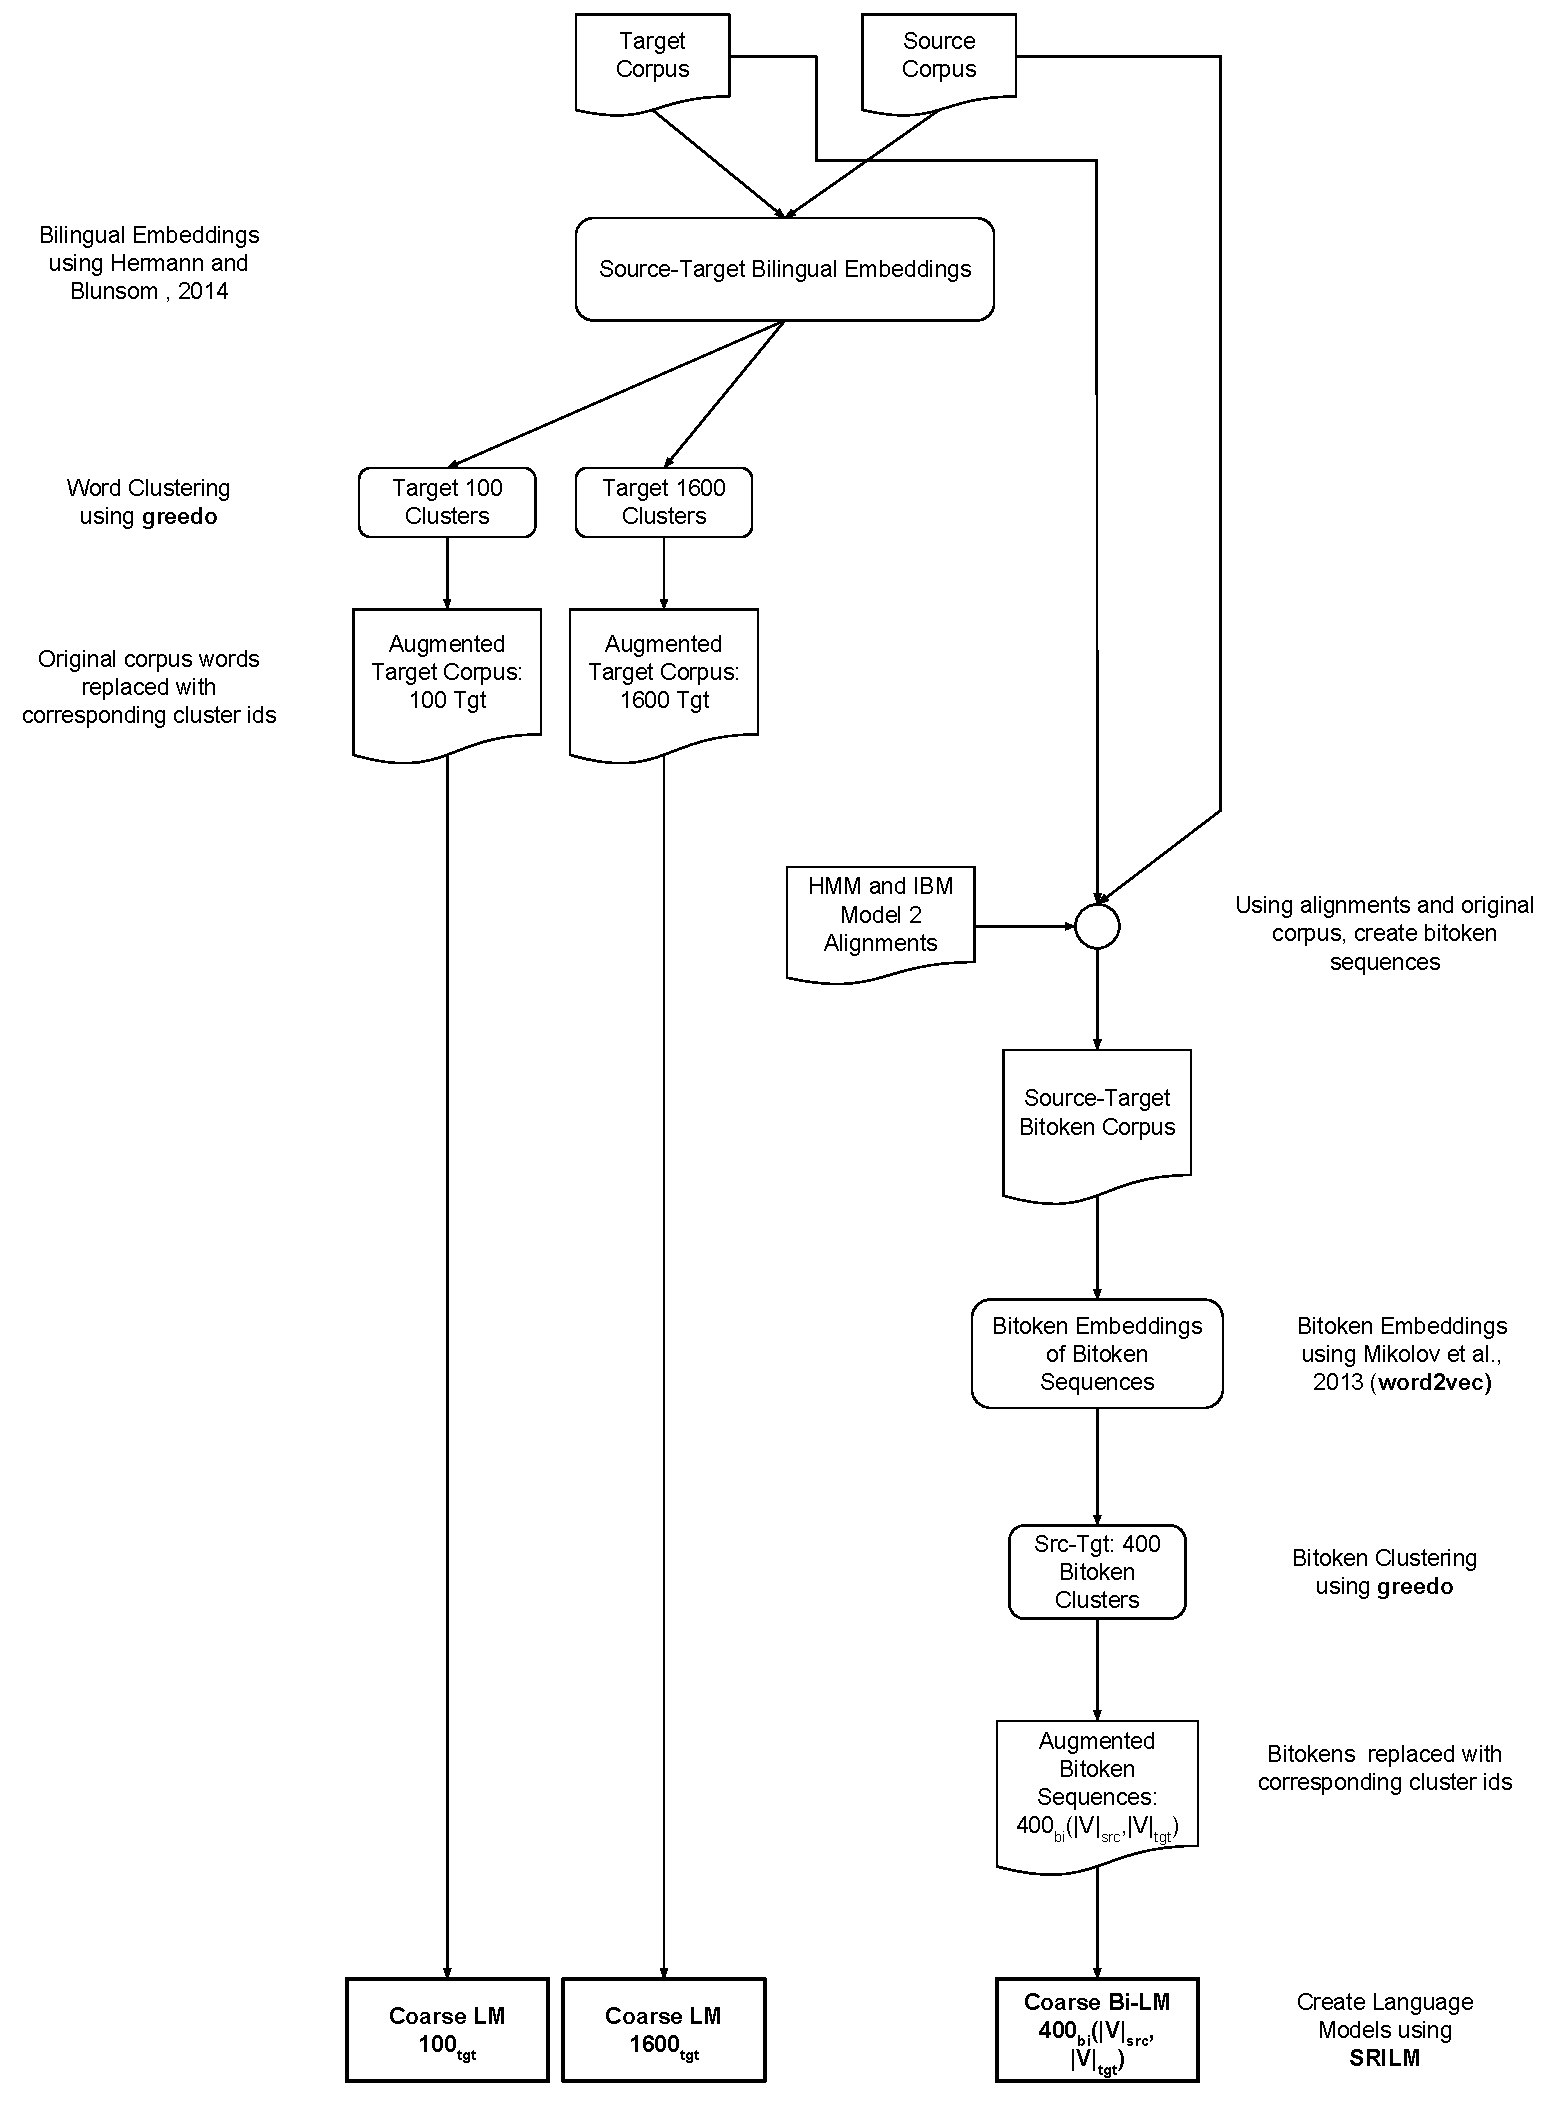
\includegraphics[width=\textwidth]{files/images/idea3}
	\end{center}
	\caption{Approach 3 for creating Coarse LMs and Coarse Bi-LMs}
	\label{fig:idea3}
\end{figure}

%\begin{figure}[htbp]
%	\begin{center}
%		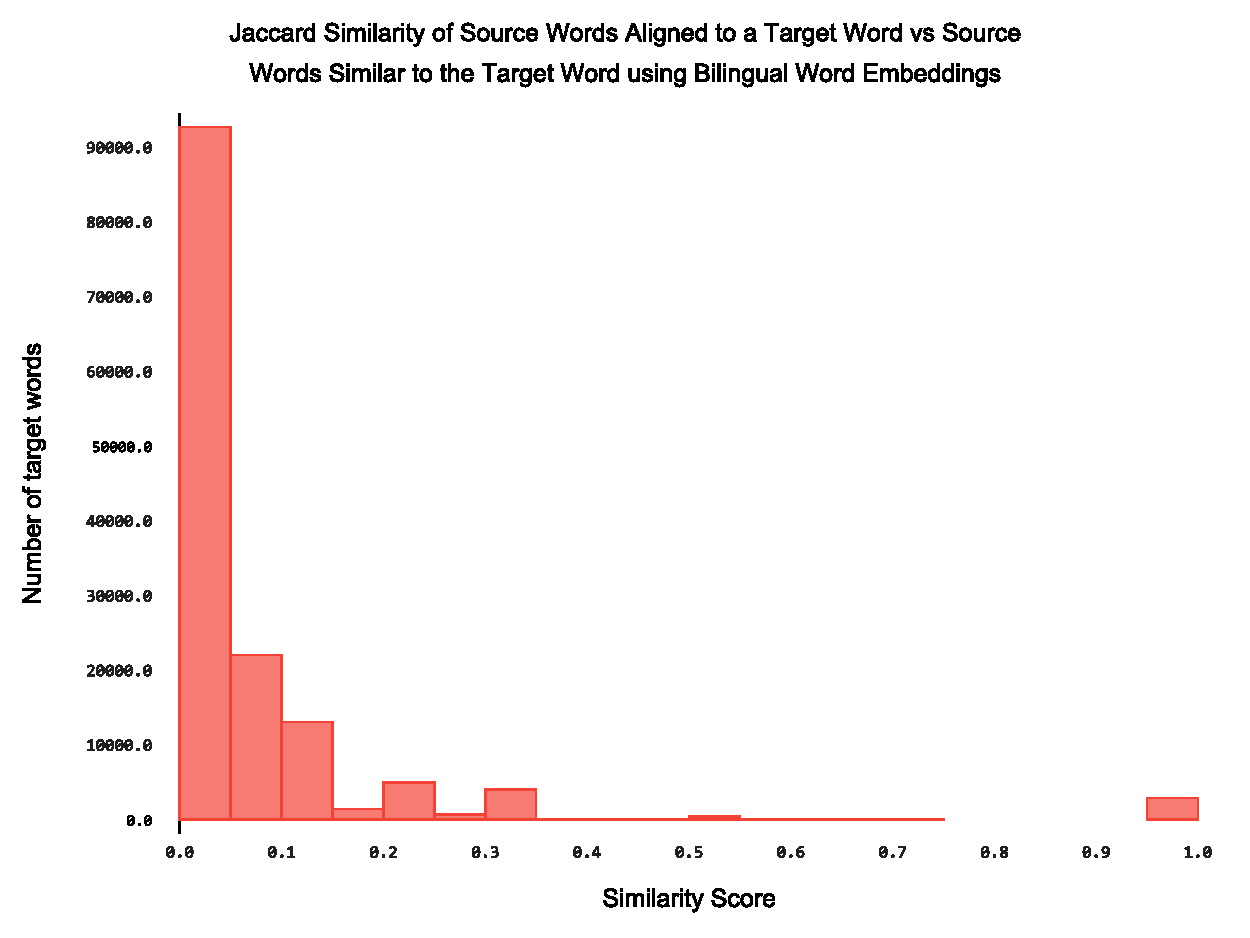
\includegraphics[width=15cm]{files/images/jaccard}
%	\end{center}
%	\caption{Jaccard similarity of source words aligned to each target word using bidirectional alignments and source words similar to the corresponding target words from bilingual word embeddings.}
%	\label{fig:jaccard}
%\end{figure}

In Chapter~\ref{three} we will discuss about the setup and how the three approaches were tested and compare the performance of the three approaches to the baseline system. In the next section we discuss about other approaches in the literature for introducing information about source words.

\section{Previous Work}
In the previous section we introduced Bi-LMs~\cite{Niehues2011,Stewart2014} and three new approaches to estimate coarse LMs and Bi-LMs. Apart from Bi-LMs, there are other approaches for introducing source side contextual information in SMT. \cite{Casacuberta2004} proposed to use stochastic finite state transducers based on bilingual n-grams. This approach was extended by \cite{Marino2006,Crego2010,Zhang2013}. \cite{Allauzen2010} successfully applied the implementation of \cite{Marino2006} on their French-English SMT task. In this approach, the translation model is implemented as a stochastic finite state transducer trained as an n-gram language model of \textit{(source, target)} pairs. When this model is trained, the source sentences are first reordered to match the order of target words using a finite state reordering model. The reordering model uses part-of-speech information to generalize reordering patterns.

\cite{Zhao2005} proposed spectral bilingual clustering for HMM (hidden markov model) based SMT~\cite{Och2003}. This model adds information of both source and target languages to the HMM model. \cite{Hasan2008} introduced a lexical trigger model for SMT in which they used triplets incorporating long distance dependencies that go beyond the local context of phrases and n-gram based language models. \cite{Feng2014} proposed factored markov backoff models along with a robust smoothing strategy that helps to generalize well. \cite{Durrani2011,Durrani2014} proposed \textit{operational sequence models (OSD)} in which they generate a sequence of source and target words and perform reordering by integrating both translation and reordering models into a single generative story. In this approach, translation decisions can influence and get impacted by reordering decisions and vice versa. This approach can be viewed as an extension to \cite{Casacuberta2004,Marino2006}.

\section{Summary}
In this chapter we introduced coarse language models and bilingual language models. We gave an in depth explaination of how bilingual language models are generated using parallel corpus and the alignments between the source and target words. We introduced the work of \cite{Niehues2011} in which he introduced part-of-speech based coarse Bi-LMs which was extended by \cite{Stewart2014} to introduce word class based coarse LMs and coarse Bi-LMs. Motivated by these approaches, we introduced our three approaches to create coarse LMs and Bi-LMs using monolingual embeddings from \textbf{word2vec}~\cite{Mikolov2013a} and bilingual word embeddings~\cite{Hermann14}. As \cite{Stewart2014} had used \textbf{mkcls} to cluster the source and target parallel corpus, we utilized \textbf{greedo}~\cite{Stratos2014} to cluster the word embeddings. Sine, both \textbf{mkcls} and \textbf{greedo} are based on the \cite{Brown1992} model of hierarchical clustering of words, this allows us to compare our approaches more coherently. In the next chapter we discuss about the setup and how we tested the three approaches and compared them to our baseline implementation of \cite{Stewart2014}.


%% Copyright 1998 Pepe Kubon
%%
%% `three.tex' --- 3rd chapter for thes-full.tex, thes-short-tex from
%%               the `csthesis' bundle
%%
%% You are allowed to distribute this file together with all files
%% mentioned in READ.ME.
%%
%% You are not allowed to modify its contents.
%%

%%%%%%%%%%%%%%%%%%%%%%%%%%%%%%%%%%%%%%%%%%%%%%%%%
%
%     Chapter 4
%
%%%%%%%%%%%%%%%%%%%%%%%%%%%%%%%%%%%%%%%%%%%%%%%%

\chapter{Experiments and Results}
\label{three}
In Chapter 2 we introduced coarse LMs and coarse Bi-LMs. We also introduced biligual word embeddings and clustering of embeddings using \textbf{greedo}~\cite{Stratos2014}. We described our baseline system, which is am implementation of \cite{Stewart2014}. We also introduced three new approaches (Section~\ref{approaches}) in which we utilize bilingual word embeddings~\cite{Hermann14} to create coarse LMs and BiLMs. In this chapter we will explain the steps that we took to test and compare our approaches to the baseline system.

For our experiments we use a Chinese(Zh)-English(En) parallel corpus. The data is separated into three parts:
\begin{itemize}
	\item The training dataset is used to train the phrase-based SMT system and bilingual word embeddings.
	\item The tuning dataset is used to tune the weights of features used in Moses decoder~\cite{Koehn2007Moses}.
	\item We report our results on the test dataset. This is a bling dataset that was not used during the training and tuning step.
\end{itemize}
Table~\ref{table:corpus-statistics} shows the details of our data.

\begin{table}
	\begin{center}
		\begin{tabular}{|c|c|c|c|}
			\hline
			\textbf{Dataset} & \textbf{Corpus} & \textbf{Size} & \textbf{Number of References}\\\hline
			Training & HK + GALE Phase 1 & 2,352,888 & N/A \\\hline
			Tuning & MTC Parts 1 \& 3 & 1927 & 4\\\hline
			Testing & MTC Part 4 & 919 & 4\\\hline
		\end{tabular}
		\caption{Corpus Statistics: Chinese-English Parallel Corpus}
		\label{table:corpus-statistics}		
	\end{center}
\end{table}

\section{Baseline System}\label{three-baseline}
Our baseline system is the system developed by \cite{Stewart2014}. As shown in Figure~\ref{fig:baseline}, we first use \textbf{mkcls} to cluster the English corpus into clusters of size 100, 400 and 1600. We also cluster the Chinese corpus into cluster of size 400. Using the English clusters, the words in English corpus are replaced with the cluster ids to create augment corporas $100_{en}$, $1600_{en}$ and $400_{en}$. Similarly, we augment the Chinese corpus using the Chinese clusters to create $400_{zh}$.

Using \textbf{SRILM}, we estimate coarse LMs \textit{Coarse LM $100_{en}$} and \textit{Coarse LM $1600_{en}$}.

To create coarse Bi-LMs, we first need to create bitoken sequences using augmented corporas $400_{zh}$ and $400_{en}$. To create the bitoken sequences, as shown in Figure~\ref{fig:bitokens-clusters}, we first need to create bidirectional alignments using the Zh-En parallel corpus. Using GIZA++\cite{Och2003}, we create the following biderectional alignments:
\begin{itemize}
	\item IBM Model 2~\cite{Brown1993} alignments.
	\item Hidden Markov Model (HMM)~\cite{Och2003} alignments. 
\end{itemize}
For both the alignments, \textit{grow-diag-final-and} heuristic (outlined in Section~\ref{intro-tm}) is used. The alignments between the source and target words in Zh-En parallel corpus from both the alignment models are concatenated together. This is done to increase the different types of bitokens. Using the alignments, and augmented corporas $400_{zh}$ and $400_{en}$, the bitoken sequences are created, called ($400_{zh}$, $400_{en}$) bitoken corpus.

A copy of the ($400_{zh}$, $400_{en}$) bitoken corpus is used to estimate coarse Bi-LM \textit{Coarse Bi-LM $(400_{zh},\ 400_{en})$}. The second copy of bitoken corpus is clustered using \textbf{mkcls} with cluster size set to 400. The bitokens in the bitoken corpus are replaced with the new cluster ids to create augmented corpus $400_{bi}(400_{zh},\ 400_{en})$ Using \textbf{SRILM}, coarse Bi-LM \textit{Coarse Bi-LM $400_{bi}(400_{zh},\ 400_{en})$} is estimated.

When estimating the coarse LMs and Bi-LMs, we use \textit{Witten-Bell smoothing} \cite{WittenBell1991}. Coarse LMs and Bi-LMs create counts of counts that the SRILM implementation of Kneser-Ney smoothing cannot cope up with. \cite{Stewart2014} states that Witten-Bell smoothing outperforms Good-Turing smoothing. They also state that 8-gram coarse models outperformed lower n-gram coarse models. Hence, all our coarse LMs and Bi-LMs are 8-gram models.

The four coarse LMs and Bi-LMs are used in a stateful feature function in Moses decoder. We will talk about decoder in a later section. In the next section we explain our steps to create the coarse models as described in our appraoches.

\section{Bi-LMs using Word Embeddings}\label{three-approaches}
In this thesis we propose three approaches to create coarse LMs and Bi-LMs (Section~\ref{approaches}). The first step in creating coarse LMs and Bi-LMs using word embeddings is to create bilingual word embeddings for Zh-En parallel corpus.

\subsection{Creating Bilingual Word Embeddings}\label{three-embeddings}
In order to create bilingual word embeddings for Zh-En parallel corpus, we use \textbf{BiCVM}~\footnote{BiCVM by Karl Mortiz Hermann: \url{https://github.com/karlmoritz/bicvm}}, which has the implementation of \cite{Hermann14}. We use the following parameters to train the embeddings:
\begin{itemize}
	\item Tree type: \texttt{plain}
	\item Type of model: \texttt{additive}
	\item Training method: \texttt{adagrad}
	\item Word vector dimensions: \texttt{word-width: 300}
	\item Hinge loss margin: \texttt{300}
	\item Number of noise samples per positive training example: \texttt{50}
	\item Step size during gradient descent: \texttt{0.05}
	\item L2 regularization for embeddings: \texttt{2}
	\item Consider bi error for language 1: \texttt{true}
	\item Consider bi error for language 2: \texttt{true}
	\item Number of training iterations: \texttt{500}
	\item Number of batches for adagrad: \texttt{50}
\end{itemize}

This will create bilingual word embeddings with 300 dimensions. We experimented with different values of parameters and different dimensions, but these parameters gave us the best embeddings. To judge how good the embeddings are, we use \textbf{WordEmbeddingsViz} (Section~\ref{WordEmbeddingsViz}). Using \textbf{WordEmbeddingsViz}, a human annotator looked at bilingual word embeddings generated with different parameters. The annotator looked at the embeddings and tried to align an English word with a Chinese word if the two words are a translation of each other. Based on observations of the human annotator, the above defined parameters for \textbf{BiCVM} were chosen. The above defined parameters were chosen because the English and Chinese word embeddings were close to each other after being projected to two dimensions using \textbf{tSNE}.

\subsection{Creating Coarse LMs and Bi-LMs using Word Embeddings}
In this subsection, we describe in detail the steps to create coarse LMs and Bi-LMs using the Zh-En bilingual embeddings (Subsection~\ref{three-embeddings}).

\subsubsection{Approach 1}
As shown in Figure~\ref{fig:idea1}, we first cluster the Zh-En bilingual word embeddings using \textbf{greedo}~\cite{Stratos2014}. The following clusters are generated:
\begin{itemize}
	\item Create clusters of size 100, 400 and 1600 for English embeddings.
	\item Create cluster of size 400 for Chinese embeddings.
\end{itemize}
Using the cluster ids for each word, we augment the corpus (as described in \ref{three-baseline}) to get augmented corporas $100_{en}$, $1600_{en}$, $400_{en}$ and $400_{zh}$. Similar to our baseline system, we estimate \textit{8-gram} coarse LMs \textit{Coarse LM $100_{en}$} and \textit{Coarse LM $1600_{en}$} using \textbf{SRILM} with \textit{Witten-Bell smoothing}. Similarly, we use HMM and IBM Model 2 alignments to create a bitoken corpus ($400_{zh}$, $400_{en}$) from augmented corporas $400_{en}$ and $400_{zh}$.

The bitoken corpus ($400_{zh}$, $400_{en}$) is clusterd using \textbf{mkcls} with cluster size set to 400. Using these clusters and bitoken corpus, augmented corpus $400_{bi}(400_{zh},\ 400_{en})$ is generated. Bitoken corpus ($400_{zh}$, $400_{en}$) and \textbf{SRILM} are used to estimate \textit{8-gram} coarse Bi-LM \textit{Coarse Bi-LM $(400_{zh},\ 400_{en})$}. Similarly, \textit{Coarse Bi-LM $400_{bi}(400_{zh},\ 400_{en})$} is estimated from augmented corpus $400_{bi}(400_{zh},\ 400_{en})$.

\subsubsection{Approach 2}
In \textit{approach 2} (Figure~\ref{fig:idea2}), we follow the same steps as in \textit{approach 1} to estimate \textit{Coarse LM $100_{en}$}, \textit{Coarse LM $1600_{en}$} and \textit{Coarse Bi-LM $(400_{zh},\ 400_{en})$}. Using \textbf{word2vec}, we create bitoken embeddings for bitoken corpus ($400_{zh}$, $400_{en}$). For \textbf{word2vec} we use continuous bag of words (CBOW) learning algorithm and the following parameters:
\begin{itemize}
	\item Initial learning rate: \texttt{0.05}
	\item Word vector dimensions: \texttt{300}
	\item Threshold for configuring which higher-frequency words are randomly downsampled: \texttt{1e-4}
	\item Negative sampling will be used and the value determines the number of noise words to be drawn: \texttt{5}
	\item Number of training iterations: \texttt{15}
	\item Maximum distance between the current and predicted word within a sentence\texttt{8}
\end{itemize}

The bitoken embeddings are clustered using \textbf{greedo} with cluster size set to 400. Utilizing the clusters, the bitoken corpus is transformed to create augmented bitoken corpus $400_{bi}(400_{zh},\ 400_{en})$. From this augmented bitoken corpus, we estimate an 8-gram coarse Bi-LM \textit{Coarse Bi-LM $400_{bi}(400_{zh},\ 400_{en})$}.

\subsubsection{Approach 3}
In \textit{approach 3}, we utilize the coarse LMs \textit{Coarse LM $100_{en}$} and \textit{Coarse LM $1600_{en}$} estimated for \textit{approach 2}. As shown in Figure~\ref{idea3}, in this appraoch we only use one coarse Bi-LM model instead of two. To

Using Zh-En parallel corpus, HMM alignments and IBM Model 2 alignments, we create a bitoken corpus ($|V|_{zh},\ |V|_{en}$). Here, $|V|$ denotes that we use the full vocabulary instead of first clustering the parallel corpus and then creating bitokens. Utilizing \textbf{word2vec} again, we create bitoken embeddings with the same parameters as used in \textit{approach 2}. The bitoken embeddings are clustered into 400 clusters using \textbf{greedo}. The clusters are then utilizied to augment the bitoken corpus to create an augmented bitoken corpus \textit{$400_{bi}(|V|_{zh},\ |V|_{en})$}. Using the augmented bitoken corpus and \textbf{SRILM}, we estimate the 8-gram coarse Bi-LM \textit{Coarse Bi-LM $400_{bi}(|V|_{zh},\ |V|_{en})$} with \textit{Witten-Bell smoothing}.

We use the coarse LMs and Bi-LMs estimated by the three approaches in Moses decoder. We describe this process in the next section.


\section{Integration with Decoder}\label{feature-function}
In Section~\ref{three-baseline} and Section~\ref{three-approaches}, we described in detail the steps to create coarse LMs and Bi-LMs. In phrase-based SMT, these models would be used as extra features in the log linear model described in Section~\ref{intro-decoder}. In Moses decoder, these features can be added by creating stateful feature functions. In the stateful feature function that we created, we use these models as language model using the KenLM~\cite{KenLM} wrapper integrated with Moses. \textbf{SRILM} stores the estimated language models in ARPA format\footnote{More details about ARPA format: \url{http://www.speech.sri.com/projects/srilm/manpages/ngram-format.5.html}}. This format is a standard format which can be read by most of the popular language modelling toolkits and specially \textbf{KenLM}. 

Using coarse LMs in a stateful feature function is straightforward. When the decoder is translating a source sentence, it create partial hypothesis for each of the possible phrases in the source sentence and their translations from the phrase table. For each partial hypothesis, all the defined feature functions are called and each of those feature functions would generate a score for the partial hypothesis. In our case, it would be log probability score by our language models. For coarse LMs, whenever the feature function is called, for each of the coarse LMs, we perform the following steps:
\begin{itemize}
	\item Extract target phrase from hypotheis.
	\item As each coarse LM was estimated for an augmented corpus, augmented by replacing words with corresponding cluster ids, we use the cluster mapping for that coarse LM to replace the words in the target phrase with the corresponding cluster id.
	\item Score the augmented target phrase using the required coarse LM.
\end{itemize}

The feature function would return the score that is calculated. This score is then used by the decoder in choosing the best possible hypothesis path while translating the sentence.

To score partial hypothesis using coarse Bi-LMs, the feature function not only uses the bilingual phrase pair in the partial hypothesis, but also uses the alignments within those phrase pairs which are available from the phrase table. Using the alignments and bilingual phrase pairs, we create the bitokens. Before creating the bitoken optionaly, we replace the words in phrase pair with the cluster ids, depending if we are calculating for \textit{approaches 1\& 2 or 3}. The bitokens are then optionally replaced by their cluster ids (they are replaced by cluster ids when estimating the score from \textit{Coarse Bi-LM $400_{bi}(|V|_{src},\ |V|_{tgt})$} and are not replaced in case of \textit{Coarse Bi-LM $(400_{src},\ 400_{tgt})$}). Once we have the set of required phrase of tokens, we can then score them with our coarse Bi-LMs.

In the next section we describe the results of the baseline system and our approaches.

\section{Results}

For our experiments as mentioned earlier we use Moses decoder~\cite{Koehn2007Moses}. We implemented a stateful feature (Section~\ref{feature-function}) function\footnote{Moses Feature Functions: \url{http://www.statmt.org/moses/?n=Moses.FeatureFunctions}} to score each partial hypothesis with the coarse LMs and Bi-LMs in the baseline system and our approaches. For all our experiments, we use a 5-gram English language model. Table~\ref{table:language-model-statistics} shows the statistics of our language model. For training the translation table, we use Moses to perform the following step on Zh-En training dataset (Table~\ref{table:corpus-statistics}):
\begin{itemize}
	\item Train alignments using GIZA++\cite{Och2003}. By default Moses will train IBM Model 4 alignments with \texttt{grow-diag-final-and} as the merging heuristic.
	\item Perform phrase extraction and scoring of features. For our experiments, we set the \texttt{max-phrase-length} setting to \textit{7} and \texttt{distortion-limit} as \textit{-1}.
	\item Create lexicalised reordering model using the heuristic \texttt{msd-bidirectional}.
\end{itemize}

This will create \texttt{moses.ini} which contains the settings of all the default features of Moses. We modify the \texttt{moses.ini} file and add information about coarse LM and coarse Bi-LMs.

For all our experiments, we tune the feature weights using \textit{Minimum Error Rate Training} (MERT)~\cite{Och2003} and BLEU score as the metric for optimization.

Table~\ref{table:results} shows BLEU scores and Translation Error Rate (TER) for the four systems. All three of our approaches consistently outperform the baseline system. \textit{Approach 2} achieves an increase of \textbf{1.4 BLEU points} over the baseline system. In the table we also report the \textit{$p$-value} of our results. The \textit{p-value} shows how statistically significant our results are. To be statistically significant, the $p$-value should be $< 0.05$, and \textit{approach 2} achieves a $p$-value of $0.00$. We used \textbf{multeval}~\cite{multeval} to calculate the BLEU score, TER score and $p$-value. Since, when looking at BLEU score \textit{approach 2} has statistically significant results, we deem it as the winning candidate out of all three of our approaches.

\begin{table}
	\begin{center}
		\begin{tabular}{|c|c|c|c|c|c|}
			\hline
			\textbf{Corpus} & \multicolumn{5}{c|}{\textbf{Counts}} \\
			\cline{2-6}
			 & \textbf{1-gram} & \textbf{2-gram} & \textbf{3-gram} & \textbf{4-gram} & \textbf{5-gram}\\\hline
			English Gigaword & 3,621,795 & 15,004,955 & 31,570,877 & 43,974,562 & 521,798,40\\\hline
		\end{tabular}
		\caption{5-gram language model for English and counts of each gram.}
		\label{table:language-model-statistics}		
	\end{center}
\end{table}

\begin{table}[htb]
	\begin{center}
			\begin{tabular}{|l|l|l|l|l|l|l|}
				\hline
				\bf Metric & \bf System & \bf Score & \bf $p$-value \\
				\hline
				\multirow{4}{*}{BLEU $\uparrow$}
				& Baseline & 23.0 & - \\
				& Approach 1 & 23.4  & 0.33 \\
				& \textbf{Approach 2} & \textbf{24.4} & \textbf{0.00} \\
				& Approach 3 & 23.1 & 0.82 \\
				\hline
				\multirow{4}{*}{TER $\downarrow$}
				& baseline & 77.5 & - \\
				& \textbf{Approach 1} & \textbf{71.0} & \textbf{0.00} \\
				& Approach 2 & 71.9 & 0.00 \\
				& Approach 3 & 73.0 & 0.00 \\
				\hline
			\end{tabular}
			\caption{Results comparing the baseline system~\ref{three-baseline} and three of our approaches~\ref{three-approaches}}
			\label{table:results}
	\end{center}
\end{table}


\section{Summary}
In this chapter we described the steps we took to implement the baseline system~\cite{Stewart2014} and our three approaches. We also describe in detail how we chose the parameters when creating the bilingual word embeddings and bitoken embeddings. Finally we show that \textbf{approach 2} outperforms the baseline by \textbf{1.4 BLEU points} and other approaches by almost \textbf{0.1 to 0.4} BLEU points. We also show that our results are statistically significant. In the next chapter we will conclude our thesis and describe where we would like to further take this research.
%%%%%%%%%%%%%%%%%%%%%%%%%%%%%%%%%%%%%%%%%%%%%%%%%
%
%     Chapter 4
%
%%%%%%%%%%%%%%%%%%%%%%%%%%%%%%%%%%%%%%%%%%%%%%%%

\chapter{Conclusion \& Future Work}\label{conclusion}

\section{Conclusion}
We started the dissertation by introducing statistical machine translation and we gave a brief overview about the steps involved in training a phrase-based statistical machine translation system using a parallel corpus. When decoding a source sentence to translate it into a target language, we show that the decoder has very little information about source words outside the current phrase pair in consideration. Little work has been done in the literature that try to incorporate information about source words outside the current phrase pair in consideration. In the quest of providing the decoder more information from words in the source sentence, \cite{Niehues2011} introduced bilingual language models. They achieved statistically significant gains by replacing words with part-of-speech tags and then creating their bilingual language models. \cite{Stewart2014} extended their work and showed that significant gains can be achieved by using a combination of coarse language models and coarse bilingual language models. \cite{Stewart2014} made their language models coarse by clustering their corpora using \textbf{mkcls}, a popular monolingual word clustering algorithm. Their approach depends on using word alignments and monolingual clusters to create the bitokens. This approach will not be able to capture the information provided by words which are not direct translations of each other as captured by word alignments. In order to include information from words which are not direct translations of each other, we proposed a novel approach of using word embeddings and bilingual word embeddings to create coarse language models and bilingual language models.

In this dissertation we present three new systems of using word embeddings and bilingual word embeddings to create coarse language models and bilingual language models. In all three systems we create bilingual word embeddings using BiCVM~\cite{Hermann14} and cluster these embeddings using \textbf{greedo}~\cite{Stratos2014}. The clusters are used to augment the Chinese-English parallel corpus. These augmented corporas are used to create coarse language models in all three of our systems. In two our systems we use augmented corporas to create bitokens, whereas in the third system we use the Chinese-English parallel corpus to create the bitokens.  In the first two systems, we create coarse bilingual language models using the bitokens itself. In all three systems, we further cluster the bitokens. We experiment with clustering the bitokens using \textbf{mkcls} and also by creating bitoken embeddings using \textbf{word2vec}. The bitoken embeddings are clustered again using \textbf{greedo}. The clusters are then used to augment the bitokens and this augmented bitoken corpus is used to create coarse bilingual language models.

In our experiments we compare our systems to a baseline system, which is an implementation of \cite{Stewart2014}. We show that all three of our systems outperform the baseline system. When looking at the BLEU score, the second system which uses coarse bilingual language models by creating bitoken embeddings performs the best and when looking at TER score, the first system which uses \textbf{mkcls} to cluster the bitokens performs the best. The second system has a $p$-value of 0.00 when looking at BLEU score, that is the improvements are statistically significant, hence we deem it as the winning system out of all three of our systems. Overall, we achieve an improvement of 1.4 BLEU points compared to our baseline system.

\section{Future Work}
\subsection{Clustering of Embeddings}
In our systems, we cluster the embeddings using \textbf{greedo}~\cite{Stratos2014}. \textbf{greedo} creates a hierarchical cluster of the embeddings by measuring the euclidean distances. As \textbf{greedo} and \textbf{mkcls} are based on \cite{Brown1992} model, it made it easier to compare our systems to the baseline system. 

Word embeddings show unique properties when we measure their similarity using cosine similarity. Word embeddings which are have a high cosine similarity tend to be semantically similar. Based on this idea, we would like to experiment with clustering algorithms that use cosine similarity as their distance measure. Specifically, we would like to experiment with using spherical k-means clustering~\cite{Hornik2012} as it uses cosine similarity as its distance measure.

\subsection{Extending Bi-LMs to Translation Model}
Even though, Bi-LMs are language models, but they act more as translation models as they do not model the fluency of target language but model the translation of source words. Based on this idea, we would like to extend the idea of using word embeddings in translation model. In phrase-based SMT, the translation model consists of phrase pairs. One way to modify the translation model to include embeddings would be to have a translation model that contains phrase embedding pairs instead of words in phrases. We would like to test this new embeddings based translation model as a standalone translation model and also as an additional translation model that complements the standard word based translation model.




%   BACK MATTER  %%%%%%%%%%%%%%%%%%%%%%%%%%%%%%%%%%%%%%%%%%%%%%%%%%%%%%%%%%%%%%
%
%   References and appendices. Appendices come after the bibliography and
%   should be in the order that they are referred to in the text.
%
%   If you include figures, etc. in an appendix, be sure to use
%
%       \caption[]{...}
%
%   to make sure they are not listed in the List of Figures.
%

\backmatter%
	\addtoToC{Bibliography}
	\bibliographystyle{apalike}
	\bibliography{files/thes-both}

%\begin{appendices} % optional
%	\chapter{Code}
%\end{appendices}
\end{document}
